\documentclass[norsk]{article}

%% Language and font encodings
\usepackage[norsk]{babel}
\selectlanguage{norsk}
\usepackage[utf8]{inputenc}
\usepackage[T1]{fontenc}
\usepackage{wrapfig}
\usepackage{booktabs}
\usepackage{parskip}
\usepackage[toc,page]{appendix}
\usepackage{icomma}
\usepackage{pdfpages}


%% Sets page size and margins
\usepackage[a4paper,top=3cm,bottom=2cm,left=3cm,right=3cm,marginparwidth=1.75cm]{geometry}

%% Useful packages
\usepackage{amsmath}
\usepackage{graphicx}
\usepackage[colorinlistoftodos]{todonotes}
\usepackage[colorlinks=true, allcolors=black]{hyperref}
\usepackage[capitalise]{cleveref} 
\crefdefaultlabelformat{#2\textbf{#1}#3}
\usepackage{url}
\usepackage{wasysym}
\usepackage{float}
\usepackage[autostyle]{csquotes}
\usepackage{makecell}
\usepackage{csquotes}
\usepackage{mhchem}
\usepackage{siunitx}
\usepackage{listings}
\usepackage{textcomp}


\definecolor{codegreen}{rgb}{0,0.6,0}
\definecolor{codegray}{rgb}{0.5,0.5,0.5}
\definecolor{codepurple}{rgb}{0.58,0,0.82}
\definecolor{backcolour}{rgb}{0.95,0.95,0.92}
\lstdefinestyle{mystyle}{
    backgroundcolor=\color{backcolour},   
    commentstyle=\color{codegreen},
    keywordstyle=\color{orange},
    numberstyle=\tiny\color{codegray},
    stringstyle=\color{codepurple},
    basicstyle=\footnotesize,
    breakatwhitespace=false,         
    breaklines=true,                 
    captionpos=b,                    
    keepspaces=true,                 
    numbers=left,                    
    numbersep=5pt,                  
    showspaces=false,                
    showstringspaces=false,
    showtabs=false,                  
    tabsize=2
}
\lstset{style=mystyle}

\renewcommand\theadalign{bc}
\renewcommand\theadfont{\bfseries}
\renewcommand\theadgape{\Gape[4pt]}
\renewcommand\cellgape{\Gape[4pt]}
\def\doubleunderline#1{\underline{\underline{#1}}}


%% Adding bibliography
\usepackage{biblatex}
\addbibresource{bibliography.bib}
\renewcommand{\baselinestretch}{1.5}

%% Appendix
\usepackage{appendix}

%% My commands, la til dem siden vi følger Hainz notasjon
\newcommand{\vecdot}[1]{\underline{\dot{\textbf{#1}}}}  
\newcommand{\vechat}[1]{\underline{\hat{\textbf{#1}}}} 
\newcommand{\mymat}[1]{\doubleunderline{\textbf{#1}}}
\newcommand{\vectil}[1]{\underline{\Tilde{\textbf{#1}}}}
\renewcommand{\vec}[1]{\underline{\textbf{#1}}}
\usepackage{textcomp}

%double underscore
\newlength\dunder
\settowidth{\dunder}{\_}
\newcommand{\twound}{\rule{2\dunder}{0.2pt}}
\DeclareSIUnit\atm{atm}
%%


%% Listing
%\usepackage{listings}
%\definecolor{mygreen}{RGB}{28,120,0}
%\lstset{
%  language=Matlab,
%  numbers=left,
 % stepnumber=1,
%  numbersep=10pt,
%  tabsize=4,
%  showspaces=false,
%  showstringspaces=false
%  breaklines=true
%  commentstyle=\color{mygreen}
%  frame = single
%}
%

\title{Kompendium i TKP4106 Prosessmodellering \\
\large{ABC på 123}}
\author{Eskild Ruud Mageli\\ Sindre Bakke Øyen}
%    \small{co-forfatter}\\
%    \small{Anders Runningen}}
%\subtitle{A closer look at the expenses}
%\subject{a funny paper}

%\date{May 2018}

\begin{document}
\thispagestyle{empty}
\vbox{
    \centering
    \maketitle
    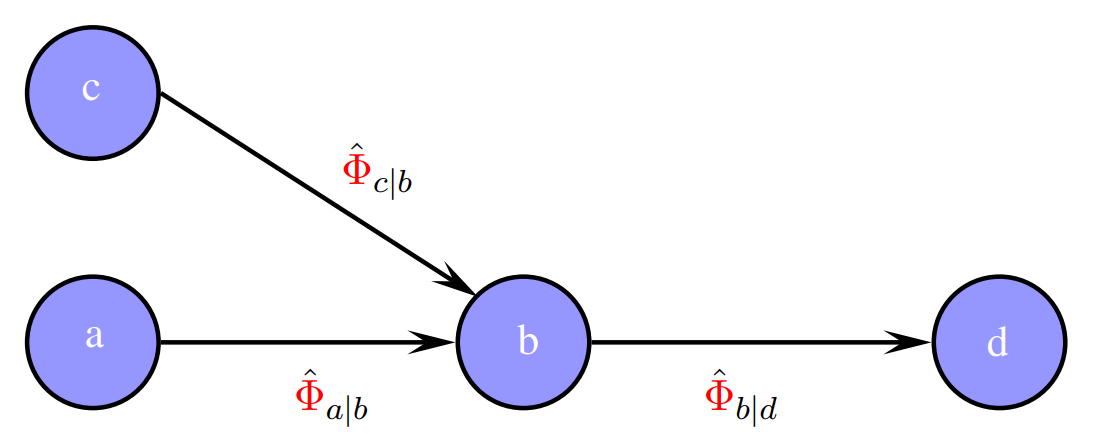
\includegraphics[scale=0.5]{Figures/massebalanser_flere_systemer} 
    

     %this typesets the contents of \title, \author and \date
}
\vfill
    \begin{center}
        \large{Kompendiumskomiteen\\ Høiskolens Chemikerforening\\komkom@hc.ntnu.no}    
    \end{center}
\thispagestyle{empty}
\clearpage
\newpage
\thispagestyle{empty}
Utforming og sideombrekking: \LaTeX \\
Illustrasjoner: Inkscape og paint.net\\
Andre illustrasjoner er printet med tillatelse fra Heinz A. Preizig. \\
Programmeringsverktøy: python 3.6.6 \\
\vfill

ABC på 123\\
\textcopyright \text{ }Eskild Ruud Mageli og Sindre Bakke Øyen 2018 \\
\email{eskild.emedd33@gmail.com} \\
\email{sindre.bakke.oyen@ntnu.no} \vfill
Høiskolens Chemikerforening har tillatelse til å distribuere bokens innhold til alle studerende medlemmer hvor innkjøpspris skal dekke kostnader for printing. Høiskolens Chemikerforening har ikke lov til selge boken for profitt men har lov til å runde prisen av boken opp til nærmerste ti-krone.

\vfill
    \Large{\textbf{Medvirkende til kompendiet}}\\
    \large{Anders Runningen\\
    Kristine Øya  \\
    Peder Langsholt Holmqvist\\
    Joachim Ågotnes 
    }
\clearpage
\begin{center}
\topskip0pt
\vspace*{\fill}
\large{Til min kjære 96-flaske}
\vspace*{\fill}


     
\end{center}
\clearpage

\section{Forord}\label{sec:forord} 
Hei og velkommen som tredjeklassing på prosess. I årene framover vil det vente deg mange morsomme, og noen krevende, emner på Institutt for kjemisk prosessteknologi. Prosessmodellering, eller prossmod, er det første av mange fag som bygger på et fundament av modellering. Ved å mestre prossmod vil de framtidige fagene bli lettere å forstå. Dette kompendiet er en slags kortversjon av faget og har som mål å være et pedagogisk hjelpemiddel til deg som student. Forelesere på IKP har nemlig en tendens til å vinkle et ellers enkelt konsept inn i vanskelige fagtermer og mange matematiske bevis. Her vil vi prøve å bruke så mange assosiasjoner som mulig, gi eksempler som du kan kjenne deg igjen i, og legge vekt på det vi mener er det viktigste å lære seg. En foreleser vil kanskje slå hardt ned på dette og si at dette ikke er korrekt på grunn av ditten og datten, men skitt au, det rette er ikke alltid pedagogisk. Kompendiet bygger på $"$The ABC of Process Modelling$"$ skrevet av Heinz Preisig. Vi presiserer at dette kompendiet ikke er offisielt pensum og gir ingen garanti for å stå i faget TKP4106 Prosessmodellering. I tillegg er det mulig faget forandrer seg med årene så kapitler i kompendiet vil ikke nødvendigvis dekke pensum fra år til år. Prossmod er et modningsfag og krever mengdetrening for forståelse, så det er viktig at du ikke tar fram dette kompendiet 3 dager før eksamen med forventning om å lære deg pensum på kort tid. Ta deg tid, gjør øvinger, diskuter faget med andre og vær kritisk til det vi skriver. Noe av det vi skriver bygger på antakelser som ikke alltid vil være realistiske, og da gjelder det å vite når man skal dykke dypere inn i emnet for en bedre forståelse. Har du spørsmål om kompendiet eller oppdager feil, så ikke nøl med å ta kontakt slik at vi kan samle opp alle endringene og eventuelt gi ut en ny utgave. Lykke til med prossmod og husk: «Hvis det går mer inn i hodet enn ut av det så akkumulerer du kunnskap». 

\setcounter{page}{1}
\clearpage


\tableofcontents

\clearpage
\clearpage-
\section{Hvordan lese dette kompendiet}\label{sec:lese}
Dette kompendiet er en kort oppsummering av pensum. Vi har valgt å bruke et uformelt språk for å gjøre kompendiet mer lettlest så du lettere skjønner konsepter. TKP4106 er undervist på engelsk (gitt at Heinz fortsatt underviser) så studentene vil ofte sitte igjen med engelske fagtermer. Vi har valgt å holde språket, men  mikser inn engelske fagtermer der vi mener det ikke finnes en god norsk oversettelse. Faget er veldig slavisk bygd opp og følger en slags oppskrift på modellering. På samme måte har vi valgt å bygge opp kompendiet med en slags $"$kokebok$"$ på hvordan man må tenke i modellering. Vi starter på overflaten og så dykker vi dypere inn i faget for å forklare hvordan man kommer fram til forskjellige ligninger. Dette innebærer at vi bruker tidligere kapitler når vi forklarer nye konsepter, så det er anbefalt å lese kompendiet fra start til slutt når du åpner kompendiet for første gang. Til tider vil du oppdage at kompendiet har mangelfulle forklaringer. Da vil vi anbefale å bruke ABC-heftet til Heinz for mer dybde. Det er også anbefalt å friske opp i fagene prosessteknikk og termo GK, samt linere algebra fra matte 3, numerikk fra matte 4N og linearisering fra matte 1. Til forskjell fra mange andre fag du har hatt tidligere er prossmod et fag hvor alle kapitler er koblet tett med hverandre. Det vil si: \textbf{IKKE PUGG}. Du kommer deg ikke gjennom prossmod ved å pugge deg til svarene siden det kreves forståelse for å bygge modeller. Selvfølgelig kan det hjelpe å pugge noen konsepter før man ser sammenhengen til andre kapitler. Men nøkkelordet vårt her er forståelse, og ferdigheten i å trekke røde tråder mellom de forskjellige kapitlene. 

\clearpage
\section{Notasjon}\label{sec:notasjon}

Før vi starter med å forklare konsepter tenker vi det er greit å gi en liten innføring i notasjonen som brukes i faget. Notasjonen kan forandre seg etter som faget utvikler seg, så ikke forvent at all notasjon er inkludert i dette kapittelet. Under har vi tatt en liten oppsummering av den viktigste notasjonsbruken i faget. For full forklaring av notasjon; se bakerst i ABC-heftet.

\begin{itemize}
    \item $\vechat{a}$: Strek under er en vektor
    \item $\mymat{A}$: To streker under er en matrise
    \item $\textbf{A}$: Tykk stor bokstav er også matrise, men sjelden brukt i dette faget.
    \item $V$: Bokstav uten strek og tykkelse er en skalar.
    \item $n$,$q$,$m$ brukes henholdsvis for stoff, volum og masse
    \item $\vecdot{n}$: Dott over $\vec{n}$ er akkumulert av $\vec{n}$ (endring av $\vec{n}$ over tid): $\frac{d(\vec{n})}{dt}$
    \item $\vechat{n}$: Hatt over $\vec{n}$ transport av $\vec{n}$.
    \item $\vechat{n}_{A|B}$: Transport av $\vec{n}$ fra A til B
    \item $\vectil{n}$: Tilde over $\vec{n}$ er generert $\vec{n}$ eller forbrukt $\vec{n}$.  
    \item $\mymat{F}^m$: En matrise som inneholder informasjon om m, i dette tilfellet er det masse og vil representere incidence matrix 
    \item \textbf{$\phi$}: Phi er brukt som ekstensiv variabel, se \cref{sec:ekstensive_intensive}
    \item \textbf{$\varphi$}: Curly phi er lik som $\phi$ men er en ekstensiv variabel som i tillegg avhenger av tid og retning. 
    \item \textbf{$\pi$}: Ikke å forveksle med tallet 3.14. Her brukes det ofte som en effortvariabel, trykk, temperatur eller kjemisk potensial, se \cref{sec:indre_effort} 
    \item := : kolon forran er-lik definerer en sammenheng.
    \item $\frac{dx}{dx}\Big|_i$: Stor strek ved siden siden av indikerer at utrykket gjelder for posisjon $i$.
    \item $\Big(\frac{\partial x}{\partial z}\Big)_{y,w}$: Derivasjon av $x$ m.h.p $z$ hvor variabel $y$ og $w$ holdes konstant.
\end{itemize}

\clearpage
\section{Topologi}\label{sec:topologi}
Kort fortalt er topologi i prossmod kunsten å dele opp et system inn i mange små kontroll volumer som $"$snakker$"$ med hverandre. En topologi inneholder ingen matematiske uttrykk, men gir en oversikt over transport av impuls, varme og/eller masse mellom de forskjellige kontrollvolumene. Hvordan vi setter opp en topologi er best forklart gjennom et enkelt eksempel, se \cref{sec:topologi_figurer}. Men før vi går igang må vi først forklare et par konsepter.

\subsection{Intensive og ekstensive variabler}
\label{sec:ekstensive_intensive}
Forskjellen mellom en intensiv og en ekstensiv variabel er at en intensiv variabel forblir uforandret når man skalerer opp systemet. Ta eksempelvis et badekar med vann. Vi antar at det fulle badekaret rommer 60 liter, og temperaturen er 25 grader. Hvis vi øker størrelsen på badekaret vil ikke lenger det fulle volumet (ekstensive variabelen) være 60 liter men temperaturen (intensive variabelen) vil fortsatt være 25 grader. 

\begin{center}
    \textit{En intensiv variabel er uavhengig av størrelsen på systemet hvor av en ekstensiv variabel vil være avhengig av størrelsen. }
\end{center}

\textbf{Eksempel på intensive variabler:} Temperatur, trykk, tetthet, kjemiskpotensial, konsentrasjon, farge, kokepunkt.

\textbf{Eksempel på ekstensive variabler:} Volum, masse, mol, entalpi, entropi, varmekapasitet, 


\clearpage
\subsection{Figurer i en topologi}\label{sec:topologi_figurer}
Her kommer det en liste med forklaringer på de vanligste figurene du støter på når du skal lage en topologi i prossmod. For full liste, se ABC-heftet. 
\begin{table}[H]
    \centering
    \begin{tabular}{c|c}
        Lumped System/Kontrollvolum & \raisebox{-.5\height}{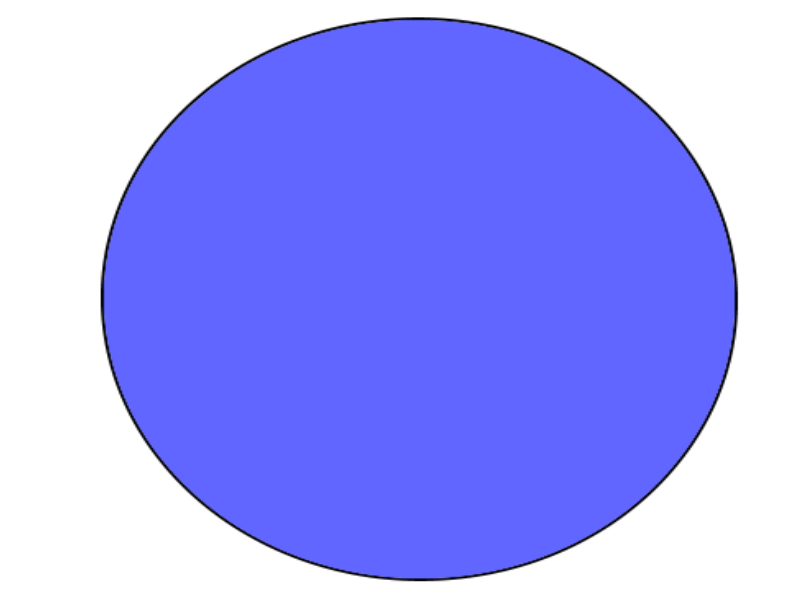
\includegraphics[scale=0.1]{Figures/Lumped.png}}\\
         Reservoar & \raisebox{-.5\height}{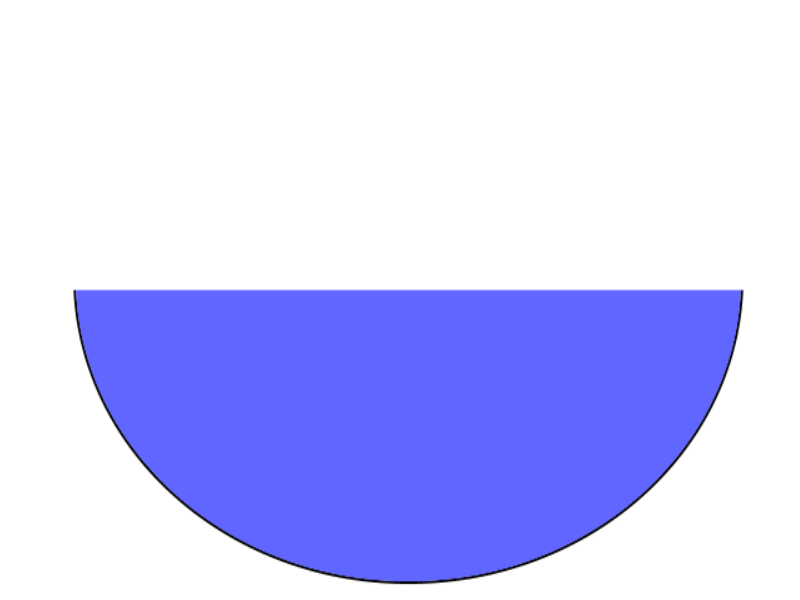
\includegraphics[scale=0.1]{Figures/Resavior.png}}\\ 
         Distributed system & \raisebox{-.5\height}{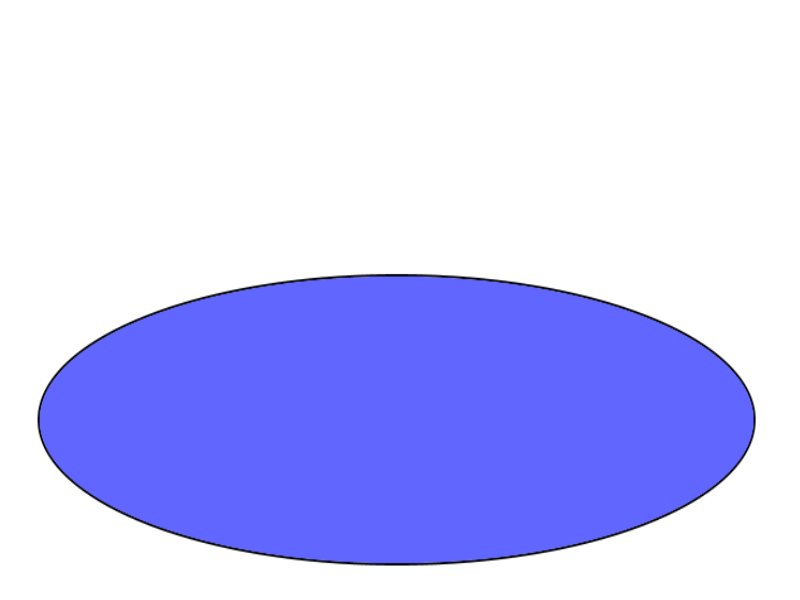
\includegraphics[scale=0.1]{Figures/Distributed.png}}\\
         Transport av masse & \raisebox{-.5\height}{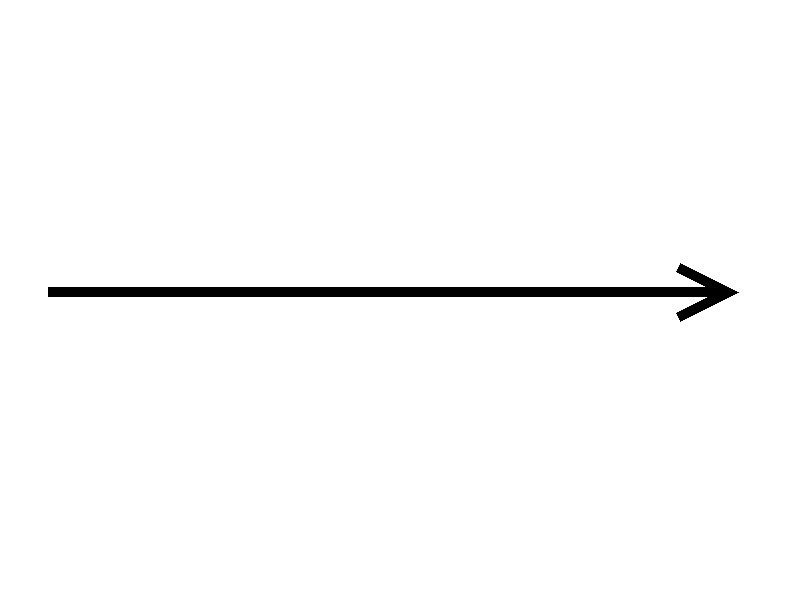
\includegraphics[scale=0.1]{Figures/mass_arrow.png}}\\
         Transport av varme (stråling, konduksjon) & \raisebox{-.5\height}{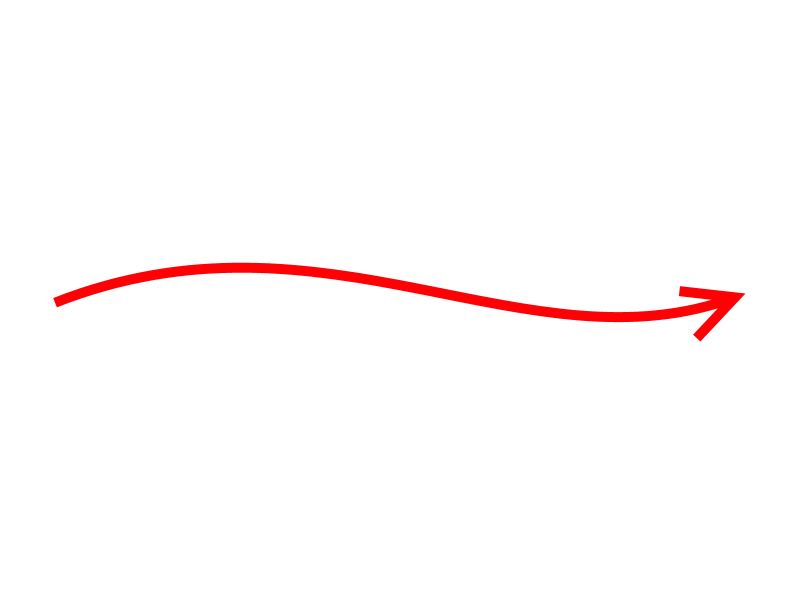
\includegraphics[scale=0.1]{Figures/Heat_arrow.png}} \\
         Transport av impuls (arbeid gjort fra et system)  & \raisebox{-.5\height}{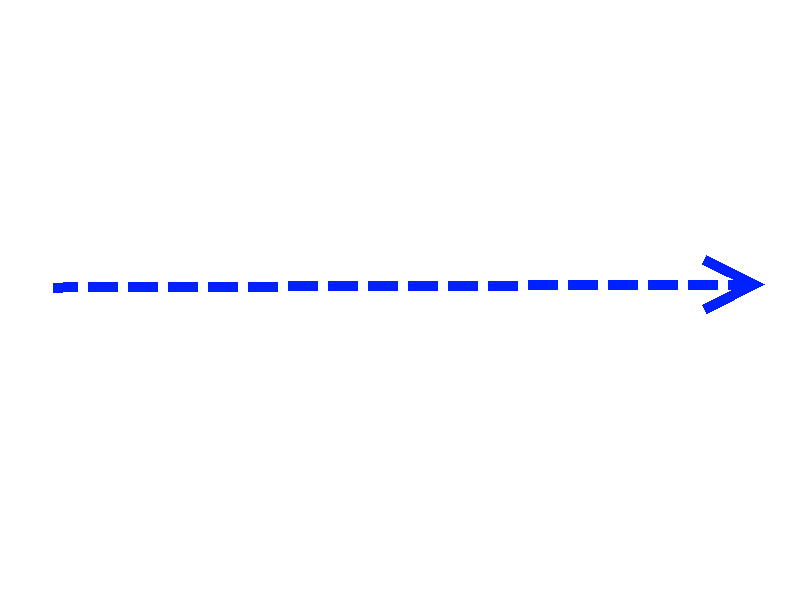
\includegraphics[scale=0.1]{Figures/Work_arrow.png}}\\
         Overflate uten kapasitet (event dynamic) & \raisebox{-.5\height}{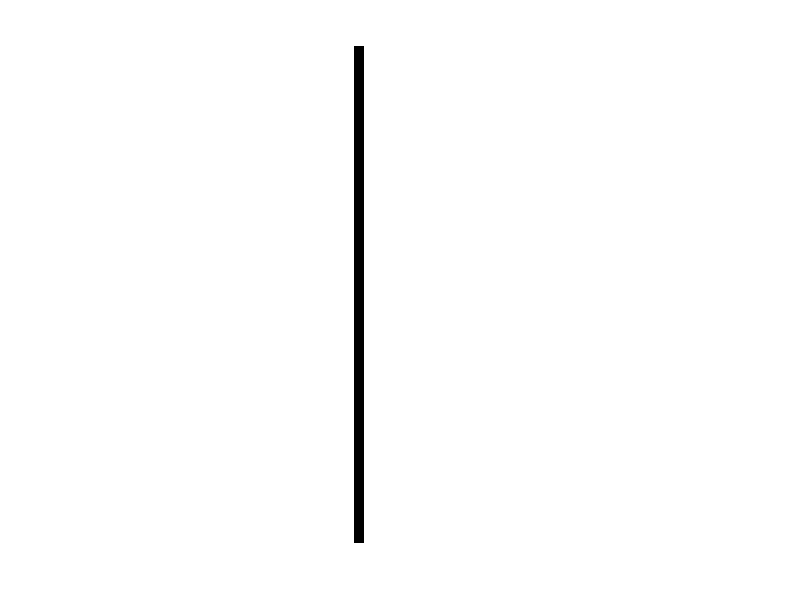
\includegraphics[scale=0.1]{Figures/surface.png}} 
    \end{tabular}
    \caption{De viktigste geometriske figurene vi finner i en topologi. For full liste, se ABC-heftet.}
    \label{tab:my_label}
\end{table}



\textbf{Lumped System}\\
Et lumped system representerer et volum/område for det fysiske systemet ditt. Ved å dele et stort system inn i mange små volumer kan vi få en grei forståelse av hvordan hver del av det store systemet kommuniserer. I et lumped system er det antatt at alle intensive variabler er isotrope. Det vil si at de intensive variablene er uavhengig av posisjon i systemet. Eksempelvis vil et målt trykk på 5 bar i volumet også være 5 bar alle andre steder i volumet. 

\textbf{Reservoar} \\
En stor menge som aldri går tom. Med andre ord vil et reservoar ha uendelig store kapasitet i form av ekstensive variabler. Når det transporteres fra eller til et reservoar vil ikke det akkumuleres i reservoaret fordi reservoaret alt har uendelig megde av den ekstensive variabelen. Alle intensive variabler i et reservoar er antatt å være konstante så et reservoar med 25 varmegrader vil forbli 25 varmegrader.

\textbf{Distributed systems}\\
Et distributed system er som et lumped system med unntak av intensive variabler avhenger av hvor vi befinner oss i systemet (anisotropt system). Eksempelvis vil temperaturen i en badstue være høyere jo lengre opp i høyden du beveger deg. Av den grunn så er kan vi ikke lenger behandle volumet av en badstue som et lumped system og må sette inn et distributed system. Merk at andre intensive variabler, som trykk og tetthet, kan være antatt konstante. Et distributed system kan være anisotrop i flere dimensjoner, men må minst være avhengig av en retning. Å modellere et distributed system er litt mer avansert, se \cref{sec:distributed}, men et lite party triks er å bruke $"$Sliced-salami$"$ metoden og dele et distributed system opp i flere mindre lumped systems. 


\textbf{Transportpiler}\\
Transportpiler er transport av ekstensive variabler fra et volum til et annet. Se \cref{sec:massetransport} for forklaring av modellering av transport. Merk at retningen på pilen er en referanse for modellen vår. Dette kan virke litt forvirrende, men det viktigste å vite er at når det transporteres fra et volum til et annet, mot pilens retning, så må vi behandle transporten som negativ. Med andre ord er det ikke pilen i seg selv som bestemmer transporten, men retningen fungerer som en referanse når vi skal bestemme hvilken vei transporten går. 

\textbf{Overflater uten kapasitet}\\
Rettere burde vi ha skrevet $"$Event dynamic systems$"$, men det er litt forvirrende første gang man hører det. Det vi prøver å få fram er at vi har et system som ikke har mulighet til akkumulering siden hendelsen går så fort. Ta eksempelvis overflaten mellom vann og gass i fordampning av vann. Overflaten mellom væsken og gassen har ingen kapasitet og selve fordampningen skjer momentant. For å forklare at væske fordamper og blir til gass i topologien vår må vi ha med et event. I det tilfellet setter vi inn en rett strek, et event dynamic system. 

 
\subsection{Eksempel: Et basseng når det regner}
Tenk deg at sjefen din nettopp har fått installert et nytt fancy basseng i hagen og han har satt deg i oppgave å fylle opp bassenget med vann. Du ser på værmeldingen for morgendagen og oppdager at det er meldt 15 mm i timen. \enquote{Woho}, tenker du, \enquote{bassenget fyller seg opp av seg selv}. Før du begynner på regndansen funderer du over hvor mye vann som samler seg i bassenget på den tiden og du undrer deg om du må fylle på med ekstra vann. Du bestemmer deg for å modellere bassenget og regnet som treffer det. Det første vi spør oss selv som ingenører er: 

\begin{center}
    \textbf{1.} Hva ønsker jeg å finne ut av?
\end{center}

I dette tilfellet er det akkumuleringen av vann i bassenget. Vi ønsker å finne ut hvor mye vann som er samlet opp i bassenget etter en viss tid. Forklart matematisk så kan vi si mengde vann i bassenget ($m_{vann}$) er integralet av akkumulert vann i bassenget ($\dot{m}_{vann}$) fra start ($t_0$) til slutt ($t$)

\begin{equation}\label{eq:integral_over_time}
    m_{vann} = \int_{t_0}^{t}\dot{m}_{vann\,}dt 
\end{equation}

\cref{eq:integral_over_time} er nå modellen vår for bassenget. Vi integrer fra $t_0$ til en $t$ også vet vi hvor mye vann som er i bassenget vårt. Desverre så har vi et problem, vi kjenner ikke hvor mye vann som akkumuleres i bassenget vårt; vi vet ikke hva $\dot{m}_{vann}$ er. Her trenger vi å sette opp en topologi. Vi må vite hvor mye vann som som kommer inn og hvor mye som går ut. Før vi kan tegne opp topologien vår må vi stille oss spørsmålene:

\begin{center}
    \textbf{2.} Hvilke antagelser tar jeg?
\end{center}

Nå som vi skal visualiserere systemet vårt gjennom en topologi må vi være klar over hvilke antagelser vi ønsker å gjøre i forkant av topologien. Et party triks i prossmod er å alltid starte enkelt også utvide topologien din ved å fjerne antagelser. I dette tilfellet vil muligens de viktigste spørsmålene være:

\begin{itemize}
    \item Lekker bassenget væske?
    \item Er det andre kilder av vann enn regnvann?
    \item Skal vi behandle all væske i bassenget som et system eller skal vi skille mellom vann og annet væske?
    \item Vil vann fordampe og gå ut fra bassenget?
    \item Skal vi bry oss om varmen i bassenget?
\end{itemize}

Først når vi er klar over hva vi neglisjerer og hva som ikke kommer fram i topologien vår kan vi skrive ned antagelsene og begynne å tegne. Her velger vi først å starte enkelt og anta at eneste kilde av væske er fra himmelen, all annen væske neglisjeres. Energibalanser ønsker vi ikke å modellere og vi antar at ikke lekker væske. 

\begin{center}
\textbf{3.} Tegn opp en topologi som reflekterer antagelsene
\end{center}

Basert på problemstillingen og antagelsene våre får vi en topologi med kun et lumped system og et reservoar. Merk at vi har valgt å se bort fra mye i starten for å få fram en enkel modell å jobbe med. Vi gjentar oss kanskje litt her, men det er fordi det er lett å forvirre seg selv. Tanken bak dette er at det er lettere å utvide en modell enn omvendt, og at det er mer strukturert å starte med det viktigste når man bygger en topologi fra scratch. 
\begin{figure}[H]
    \centering
    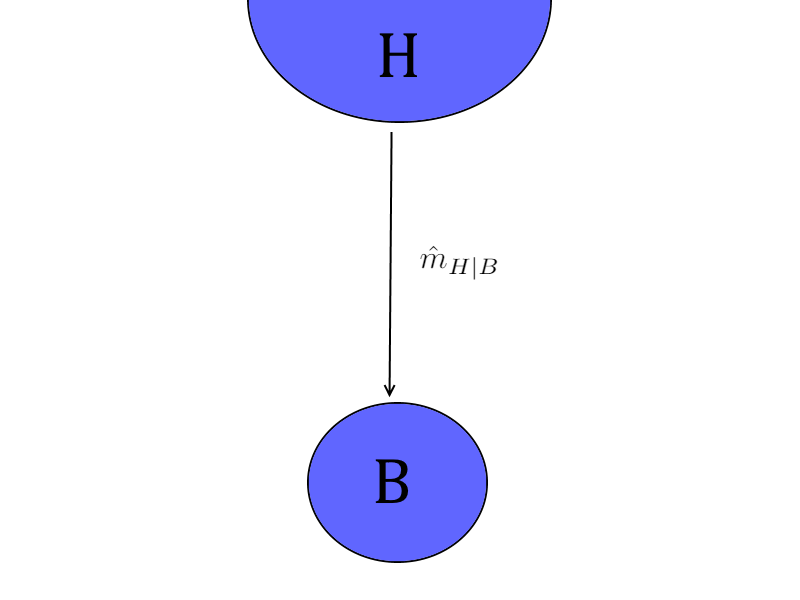
\includegraphics[scale=0.3]{Figures/Basseng1.png}
    \caption{Topilogi av regnvann inn i et basseng, H representere himmel og B representerer basseng.}
    \label{fig:topologi_enkel1}
\end{figure}

I \cref{fig:topologi_enkel1} ser vi representasjonen av massetransport fra H (himmel) til B (basseng). I denne topologien ser vi at all akkumulering av masse i B skyldes transporten fra H til B ($\hat{m}_{H|B}$). Nå som vi har en enkel modell kan vi vurdere hvorvidt vi skal utvide den eller ikke. Husk at en modell vil aldri være perfekt og det er bedre å ha en enkel modell som er god nok enn en vanskelig  modell som knapt forbedrer.  

\begin{center}
    \textbf{4.} Kan/bør jeg utvide topologien min?
\end{center}

 Topologien er på plass, livet er fint, men så kommer sjefen din og oppdager planen din om å la regnet gjøre arbeidet. Han fnyser av deg, men aksepterer  arbeidet ditt mot at du også skal ta hensyn til lekkasje og fordampingen av vann i bassenget. $"$Fillern$"$ tenker du og hopper tilbake til arbeidet. Når vi utvider en modell er det viktig å gå tilbake på antagelsene og revurdere dem før vi utvider. For å få fram fordampningen og for å vise at bassenget vårt består av et volum av væske og et volum av gass setter vi opp to lumped systems med et event dynamic system mellom seg (overflaten). I tillegg antar vi at lekkasjen av væske skjer til bakken og at luften i bassenget forsvinner ut til omgivelsene.  
 
 \begin{figure}[H]
     \centering
     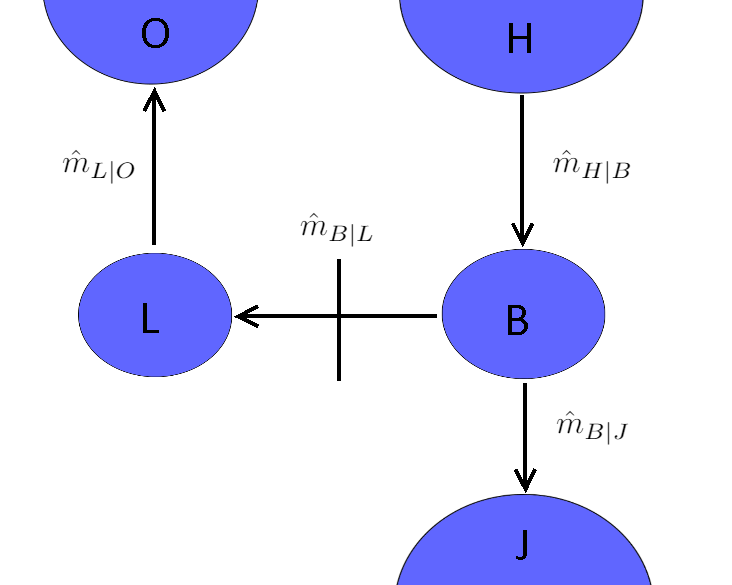
\includegraphics[scale=0.3]{Figures/Basseng2.png}
     \caption{Topologi av et basseng. H er en regnfull himmel, B er vannet i bassenget, L er luften i bassenget, O er luften i omgivelsene rundt bassenget, J er bakken.}
     \label{fig:basseng_vanskelig}
 \end{figure}

Den nye topologien er på plass og livet er nok en gang fint. Vi har laget en topologi hvor vi kan lage balanser rundt to volumer. Sjefen vår er ikke helt fornøyd og forventer at vi samtidig må ta hensyn til varmen i modellen vår. Vi sukker dypt, men etter litt tankegang kommer vi fram til en vår endelige topologi:

\begin{figure}[H]
    \centering
    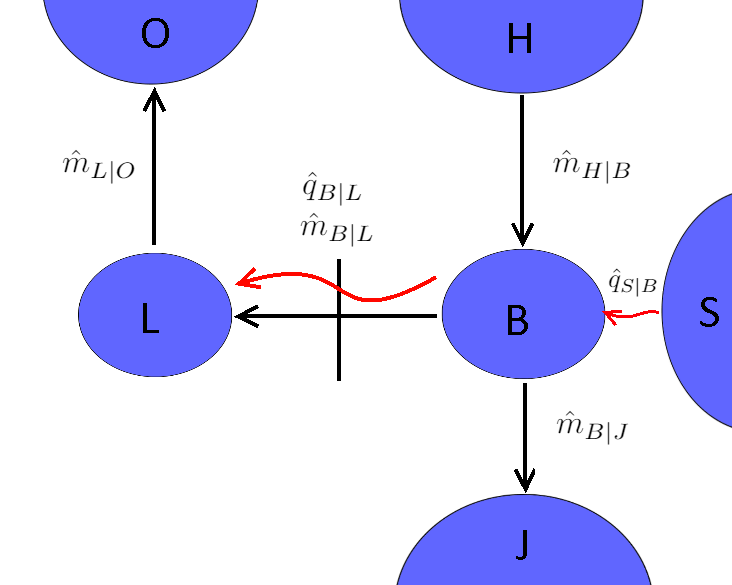
\includegraphics[scale=0.3]{Figures/Basseng3.png}
    \caption{Topologi av et basseng. H er en regnfull himmel, B er vannet i bassenget, L er luften i bassenget, O er luften i omgivelsene rundt bassenget, J er bakken, S er solen}
    \label{fig:my_label}
\end{figure}
I denne topologien har vi antatt at solen er den eneste reservoaret av varme. Vi har neglisjert oppvarming av luften fra sola. Varmetransporten mellom B og L skyldes at hvis B skal fordampe kreves det energi i form av fordampningsentalpi. Det er ingen varmetransport fra bakken til jorden selv om molekylene i bassenget har blitt varmet opp av sola. Dette skyldes at lekkasjen transporterer varme i form av konveksjon som i termodynamikken regnes som transport av indre energi, mer om dette i \cref{sec:konveksjon_konduksjon}. Heldigvis er vi nå ferdig med topologien vår. Vi leverer arbeidet vårt til sjefen som ser seg fornøyd og spanderer en Big Mac på oss. 

\begin{center}
    \textbf{5.} Ingen topologier er perfekte
\end{center}

Nå som vi har laget en topologi og ønsker å bruke den til å lage en matematisk modell for volumet i bassenget er det viktig å være klar over begrensninger til modellen vår. For eksempel er det godt mulig at antagelsen vår om at isotropisk oppførsel for temperaturen i bassenget og luften ikke er en god antagelsen. En mulighet kunne vært å sette inn et distributed system istedet, men det ville samtidig komplisere modellen vår. Ved å være klar over hva topologien ikke fremstiller er vi også klar over hvilke begrensninger modellen vår har når vi bruker den. Å vite hva som er svakhetene til en modell er essensielt siden du ikke har LF ute i arbeidslivet. 

\subsection{Oppsummert: Hvordan lage en topologi}
\begin{enumerate}
    \item Finn ut hva du ønsker å finne ut av. Er det modellering av masse, energi, impuls eller en kombinasjon?
    \item Hvilke antagelse er fornuftige? Start med det essensielle for problemet
    \item Tegn opp en topologi som reflekterer antagelsene
    \item Utvid topologien og modellen til du har en \enquote{god nok} representasjon av det fysiske systemet ditt
\end{enumerate}

\clearpage
\clearpage
\section{Representere et system med ligninger}\label{sec:massetransport}


Når vi snakker om å representere et system med ligninger mener vi å sette opp balanseligninger. I prossmod er det et fåtall av ligninger du trenger å kunne, men en av de viktigste er hvordan vi setter opp en balanse for et lumped system/kontrollvolum.
\begin{equation}
    \label{eq:akkumulering_generell}
    Akkumulering = Inn - Ut + Generert 
\end{equation}

Kort fortalt ønsker vi å sette opp en ligning for hvordan en ekstensiv variabel endrer seg inne i volumet. Fra \cref{eq:akkumulering_generell} ser vi at endringen inne i volumet er avhengig av transporten inn og ut, og hvor mye som genereres/forbrukes inni volumet. Merk at vi bare kan sette opp en slik balanse for ekstensive variabler siden intensive variabler er uavhengig av størrelsen på systemet. Vi bruker variabelen $\Phi$ som en vilkårlig ekstensiv variabel videre i kapittelet.  

\subsection{Balanser og konservering}\label{sec:balanser_konservering}
\begin{align} \label{eq:konservering_generell}
    \text{Konservering: }\dot{\Phi}_{system} &= \hat{\Phi}_{inn} - \hat{\Phi}_{ut} \\
    \label{eq:balanse_generell}
    \text{Balanse: }\dot{\Phi}_{system} &= \hat{\Phi}_{inn} - \hat{\Phi}_{ut} + \Tilde{\Phi}_{system}
\end{align}

En konservering er en balanse hvor genereringen av den ekstensive variabelen er null, dvs. all akkumulering skyldes transport inn og ut av systemet. Et system kan ofte bestå av balanser og konserveringer. For eksempel i en reaktor vil det genereres stoffmengde, men den totale massen vil være konservert.  Du kommer deg fint gjennom livet ved bare å bruke terminologien balanser, men vær klar over at en balanse blir en konservering når det ikke er generering/forbruk, det vil si $\Tilde{\Phi}_{system}$ = 0. For å ikke forvirre leseren vil vi bruke terminologien balanse videre i kompendiet.

\subsection{Sette opp en enkel balanse fra en topologi} \label{sec:balanse_enkel}

\begin{figure}[H]
    \centering
    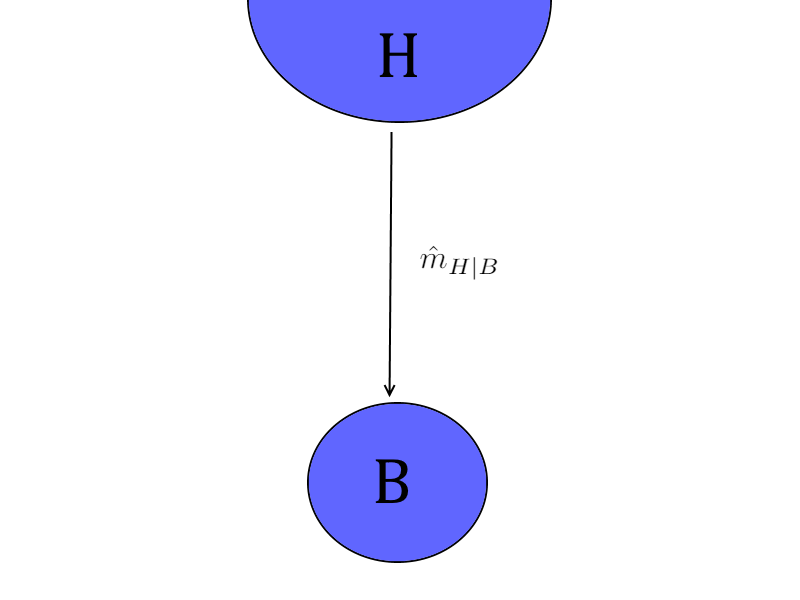
\includegraphics[scale=0.3]{Figures/Basseng1.png}
    \caption{Topologi av regnvann inn i et basseng, H representere himmel og B representerer bassenget.}
    \label{fig:topologi_enkel2}
\end{figure}
Det er kun rundt systemer med kapasitet vi kan gjøre balanser (lumped/distributed). I vår topologi, gitt i \cref{fig:topologi_enkel2}, er H et reservoar og er ikke interessant å gjøre en balanse rundt siden kapasiteten er uendelig ($\dot{\Phi}_H=0$). Volumet B kan vi sette opp en balanse rundt ved å bruke \cref{eq:balanse_generell}:

\begin{equation}
    \dot{\Phi}_{B} = \hat{\Phi}_{H|B}
\end{equation}

Vi vet alt at vår ekstensive variabel fra topologien er masse så kan vi bytte ut $\Phi$ med $m$:


\begin{equation}
    \dot{m}_B = \hat{m}_{H|B}    
\end{equation}
Vi har nå en ligning for systemet vårt og vi kan regne ut akkumuleringen av masse i B hvis vi vet transporten fra H til B. 

\subsection{Eksempel: Sette opp balanser for flere systemer}\label{sec:flere_massebalanser}
\begin{figure}[H]
    \centering
    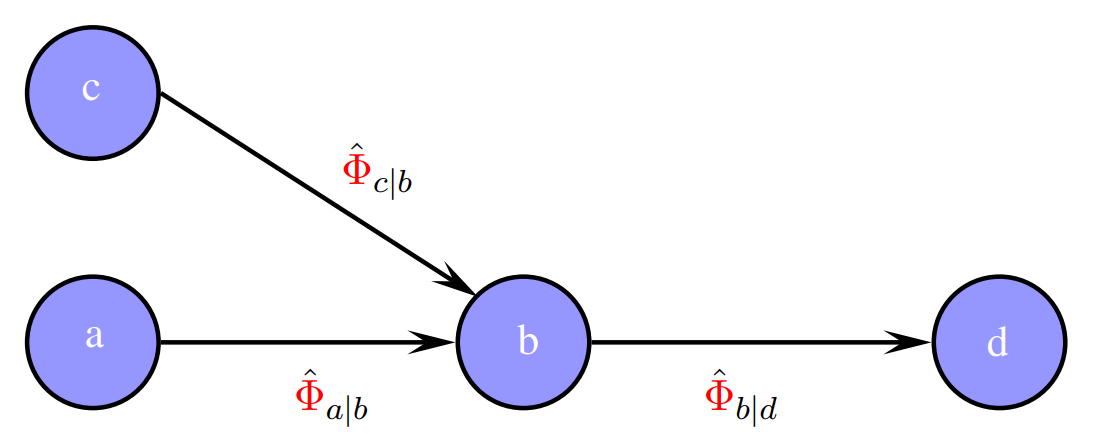
\includegraphics[scale=0.3]{Figures/massebalanser_flere_systemer}
    \caption{Topologi av fire lumped systems med transport av en ekstensiv variabel. Figur hentet fra ABC-heftet.}
    \label{fig:massebalanser_flersystem}
\end{figure}
Vi har et system bestående av fire lumped systems. Ved å benytte oss av samme teknikk som i kapittel \ref{sec:balanse_enkel} setter vi opp fire balanser: 
\begin{equation} 
    \begin{split}
    \label{eq:massebalanser_vanskelig1}
    \dot{\Phi}_{a} = & -\hat{\Phi}_{a|b} \\
    \dot{\Phi}_{b} = &\hspace{0.1cm} \hat{\Phi}_{a|b} + \hat{\Phi}_{c|b}-\hat{\Phi}_{b|d}\\
    \dot{\Phi}_{c} = & -\hat{\Phi}_{c|b}\\
    \dot{\Phi}_{d} = & \hspace{0.1cm}\hat{\Phi}_{b|d} \end{split}
\end{equation}


\subsection{Incidence matrix}
I modellering får vi ofte et system som består av flere titalls mindre systemer som gjør det vanskelig å holde styr på alle balansene. Det er derfor ønskelig å benytte seg av vektorer og matriser. 

Ved utgangspunkt i (likningssett) \ref{eq:massebalanser_vanskelig1} definerer vi vektoren for akkumulering og transport:\\ 
\begin{center}
    Vektor for akkumulering: $\underline{\dot{\Phi}}$ =
$[\dot{\Phi}_a,\dot{\Phi}_b,\dot{\Phi}_c,\dot{\Phi}_d]$ \\
Vektor for transport:  $\underline{\hat{\Phi}}$ =
$[\hat{\Phi}_{a|b},\hat{\Phi}_{c|b},\hat{\Phi}_{b|d}]$
    
\end{center}

Vi bruker disse vektorene til å representere balansene fra (likningssett) \ref{eq:massebalanser_vanskelig1} i en samlet matrise som har navn \textit{Incidence Matrix}.

\begin{equation}
    \textbf{\doubleunderline{F}} = 
    \bordermatrix{~ & \hat{\Phi}_{a|b} & \hat{\Phi}_{c|b}  & \hat{\Phi}_{b|d} \cr
                  \dot{\Phi}_a & -1 & 0 & 0 \cr
                  \dot{\Phi}_b & +1 & +1 & -1\cr
                  \dot{\Phi}_c & 0 & -1 & 0\cr
                  \dot{\Phi}_d & 0 & 0 & +1
                  }
\end{equation}
Hver rad i incidence matrix representerer en balanse og hver kolonne representerer transport fra et volum til et annet. Ved å sette opp incidence matrix kan vi skrive likningsettet \ref{eq:massebalanser_vanskelig1} som:

\begin{equation}
   \underline{\dot{\Phi}} = \textbf{\doubleunderline{F}}\hspace{0.1cm}\underline{\hat{\Phi}}
\end{equation}

Her har vi nå satt sammen et likningsett inn til en ligning med vektorer og matriser. Senere i kompendiet vil vi fortsette med denne notasjonen for å vise den lineære algebraen som kommer fram når vi modellerer. Bakgrunnen for å bruke denne notasjonen fremfor å forklare det med likninger er fordi lineær algebra har strengere krav for operasjoner enn operasjoner på skalarer i en enkel likning. Hvis du nå tenker ``Men jeg husker ikke så mye fra Matte 3'', sorry brah! Lineær algebra kommer du deg ikke utenom på IKP. Likevel, hvis du føler det er vanskelig å forholde seg til notasjonen så kan det hjelpe å skrive ut matrisen til et sett med ligninger og forholde seg til dem istedet. 

\clearpage
\subsection{Blokkmatriser}
Når man skal sette opp en incidence matrix for flere komponenter, e.g. stoffmengder, kan det være lurt å bruke matrisen til å sette opp en blokkmatrise. Dette er vanlig når man har flere komponenter som beveger seg mellom forskjellige volum. 

\begin{figure}[H]
    \centering
    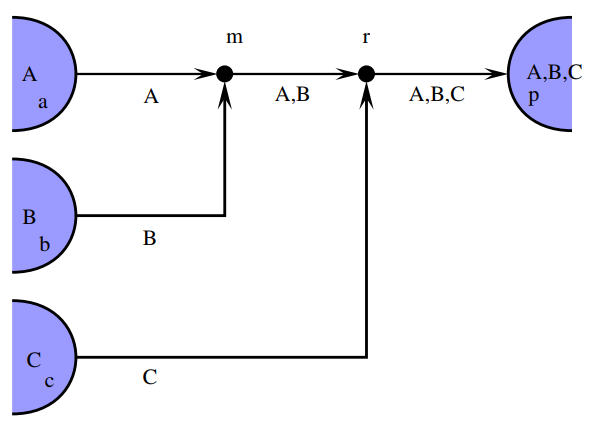
\includegraphics[scale=0.7]{Figures/Block_matrix_topo}
    \caption{Topologi av system m og r som transporerer stoffene A,B og C. Figur hentet fra ABC-heftet.}
    \label{fig:block_matrix1}
\end{figure}

\begin{figure}[H]
    \centering
    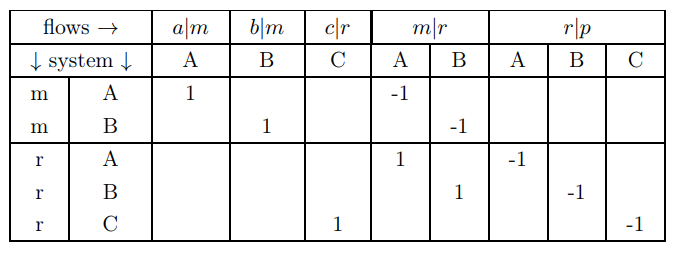
\includegraphics[scale=0.7]{Figures/Block_matrix}
    \caption{Incidence block matrix for topologien presentert i  \cref{fig:block_matrix1}. Figur hentet fra ABC-heftet.}
    \label{fig:block_marix}
\end{figure}
Vi dekker ikke denne delen i kompendiet siden prinsippet er mye av det samme, men oppfordrer sterkt å lese kapittel 7.1 i ABC-heftet hvis du ikke forstår deg på blokkmatriser.



\clearpage
\section{Transport og drivende kraft}\label{sec:transport_effort}
Til nå har vi antatt at vi kjenner transporten mellom hvert system. Hva gjør vi hvis vi ikke kjenner denne transporten? Svaret er kanskje ikke overraskende; Vi modellerer den! Men hvordan modellerer vi transporten ($\hat{\Phi}_{a|c}$, $\hat{\Phi}_{b|c}$, $\dots$) mellom de forskjellige systemene? Spenn setebeltet fast for nå beveger vi oss inn i termodynamikken.

\subsection{Indre energi og effortvariabler}\label{sec:indre_effort} Endringen av en ekstensiv variabel $\hat{\Phi}$ er bestemt av intensive variaber. Vi gidder ikke bruke mye tid på å forklare all matematikken bak drivende kraft (Kapittel 5.1 i ABC-heftet) så vi hopper rett inn i det som kalles \textit{effortvariabler} ($\pi$). Effortvariabler er intensive variabler definert som endringen av indre energi U ved forskjellige kriterier. Indre energi er en funksjon av entropi, volum og stoffmengde (S,V,\underline{\textbf{n}}) som vi finner i ligningen for total energi. I ligningene under ser vi sammenhengen mellom indre energi og effortvariabler.  Notasjonen med underindekser til brøken betyr at de variablene holdes konstant.

\begin{equation}
\label{eq:indre_energi}
\begin{split}
\Big(\frac{\partial U}{\partial S}\Big)_{V,\underline{\textbf{n}}} =:&\hspace{0.1cm} T \\
\Big(\frac{\partial U}{\partial V}\Big)_{S,\underline{\textbf{n}}} =:&\hspace{0.1cm} -p \\
\Big(\frac{\partial U}{\partial \underline{\textbf{n}}}\Big)_{S,V} =:&\hspace{0.1cm} \mu
\end{split}
\end{equation}

Det viktigste å huske fra Ligningene i \ref{eq:indre_energi} er at temperatur, trykk og kjemisk potensial er effortvariablene som sørger for endringer i ekstensive variabler. Med andre ord er det endring i T, p og $\mu$ som sørger for transport fra et system til et annet. For eksempel vil varmetap i en bolig skje fordi temperaturen utenfor er lavere enn temperaturen inne. Det vil si at forskjellen mellom temperaturen ute og inne sørger for transport av varme ut fra boligen. 

\textbf{Ekstra}:\\ 
Konsentrasjon og molbrøk er ikke effortvariabler, men istedet utledet fra kjemisk potensial. Ofte brukes konsentrasjon i uttrykk for transporten i form av diffusjon eller kjemisk reaksjon. Det er ikke nødvendigvis feil å bruke konsentrasjon i beregningene, men ved likevekt vil ikke nødvendigvis konsentrasjonsforskjellen mellom de to stoffmengdene være null, men forskjellen i det kjemiske potensialet vil alltid være null.  

\subsection{Konduksjon VS konveksjon}\label{sec:konveksjon_konduksjon}
Dette er to ord som ofte blir brukt om hverandre i varmetransport og som kan forvirre mange. 

\begin{itemize}
    \item \textbf{Konduksjon}: overføring av varme fra et molekyl til et annet via gnisninger mellom molekylene
    \item \textbf{Konveksjon}: varmeoverføring på grunn av transport av masse med høy indre energi
\end{itemize}
Eksempel på konvenksjon er kulden du merker når du åpner et vindu på en kald vinterdag. Alle de kalde luftmolekylene, med lavere indre energi enn molekylene i rommet, transporteres inn i stuen din og kjøler deg ned. Konduksjon er transporten av varmen gjennom veggen og ut til den kalde luften. Hvorfor er dette viktig å vite, spør du. Jo, for når du skal tegne opp en topologi for varmetransport vil ikke konveksjon behandles likt som konduksjon i en modell. Konveksjon behandles som transport av indre energi (som oftest entalpi). Men ikke tenk for mye på dette. PS: Stråling er også en form for varmetransport som du sikker husker fra Strømningsfaget. 

\subsection{Generell transportlov}
Hvis vi har transport av en ekstensiv variabel fra et system til et annet hvor posisjonen i system er betydelig for transporten ($\hat{\varphi}$), så er det vanlig å sette opp en differensialligning for endringen av effortvariabelen. NB: her bruker vi $\hat{\varphi}$ istedet for $\hat{\Phi}$ siden den ekstensive variabelen er avhengig av posisjon.

\begin{equation}
    \label{eq:transport_lov}
    \hat{\varphi} = -c\frac{\partial \pi}{\partial \underline{\textbf{r}}}
\end{equation}
$c$ er konduktiviteten (utrykk for mostanden) og $\underline{\textbf{r}}$ er retningene som $\hat{\varphi}$ transporteres gjennom. Denne ligningen ligner på Ficks lov eller Fouriers lov som du, forhåpentligvis, har sett tidligere i henholdsvis RekTek og Termo GK. Til vår glede er \cref{eq:transport_lov} Ficks og Fouriers lov på generell form. 

\textbf{Eksempel:}\\
Si at vi har en topologi som er representert med to lumped systems med transport mellom de to systemene, se \cref{fig:transport_topologi1}. 

\begin{figure}[H]
    \centering
    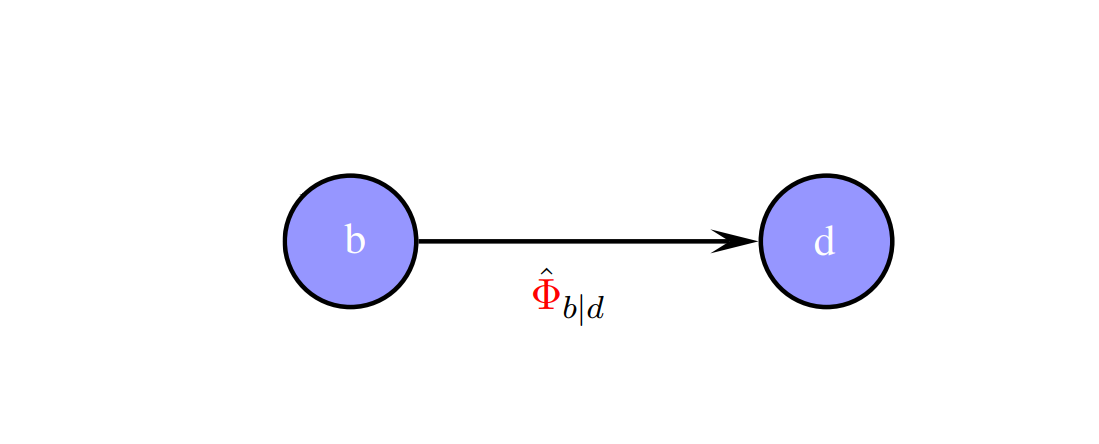
\includegraphics[scale=0.3]{Figures/Transport_topologi.png}
    \caption{Topologi av to lumped systems med transort fra $b$ til $d$.}
    \label{fig:transport_topologi1}
\end{figure}

Bruker vi \cref{eq:transport_lov} for transporten mellom $b$ og $d$ ser vi at transporten, $\hat{\Phi}_{b|d}$, er avhengig av endringen av $\pi$ i system $b$ og $d$: 
\begin{equation}
\hat{\Phi}_{b|d} = \hat{\varphi}_{b|d} = -c_{b|d}\frac{\partial \,( \pi_{b|d})}{\partial \, r_{b|d}}
\end{equation}

\subsection{Lineær modell for transport}\label{sec:linear_transport}
Anta at vi er interessert i en enkel modell for transporten mellom $b$ og $d$, som vist i Figur \ref{fig:transport_topologi1}, og ikke har informasjon om hvordan $\pi$ endrer seg fra $b$ til $d$. Da er det rimelig å benytte seg av en lineær modell for transporten mellom systemene. Vi lineariserer endringen av effortvariablen fra system $b$ til $d$ og får en modell som er grafisk representert i \cref{fig:linearized_transport}. 

\begin{figure}[H]
    \centering
    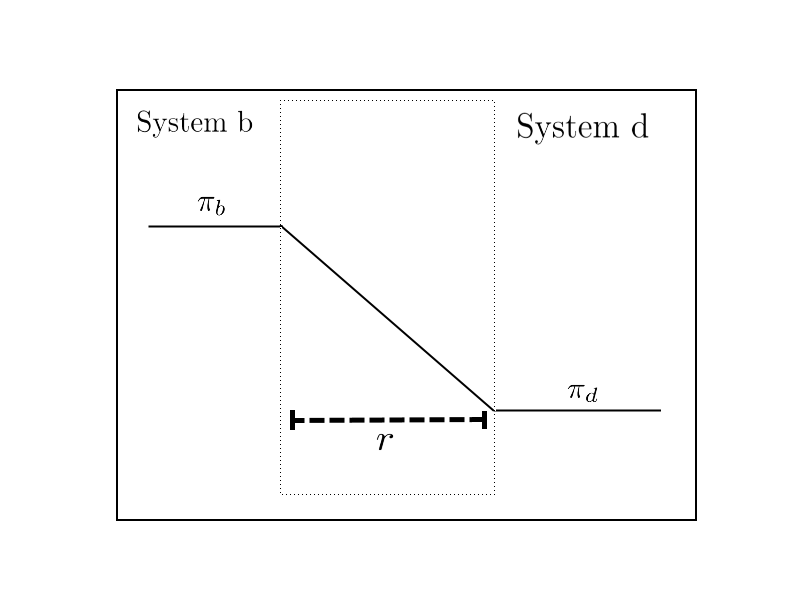
\includegraphics[scale=0.5]{Figures/linearized_transport.png}
    \caption{Grafisk representasjon av lineariseringen av $\frac{\partial \pi}{\partial \underline{\textbf{r}}}$  som viser den lineære endringen i effortvariabelene fra system $b$ til system $d$. $r$ er avstanden mellom systemene. }
    \label{fig:linearized_transport}
\end{figure}
Lineariseringen av $\frac{\partial \pi}{\partial \underline{\textbf{r}}}$ gjøres ved bruk av en Taylor utvidelse av første orden, se \cref{sec:distributed}. Dette gir oss en lineær modell for transporten av den ekstensive variabelen:



\begin{equation}
    \label{eq:transportlov_linear}
    \hat{\Phi}_{b|d} = -k_{b|d}(\pi_b-\pi_d)
\end{equation}

Denne ligningen kan vi nå substituere inn i balansene fra  \cref{sec:massetransport}. Merk at vi har en lineær modell som ikke nødvendigvis er korrekt. Hvis transporten mellom to systemer er essensielt for modellen kan det være lurt å benytte seg av andre metoder for modellering av transport f. eks. \cref{eq:transport_lov}, Governing equations (ikke pensum), Navier Stokes (ikke pensum) eller shell balance. 


\clearpage
\section{Reaksjoner og reaksjonskinetikk}\label{sec:kinetics}
Reaksjoner sies å være fundamentet i kjemisk industri. Reaksjoner er interaksjoner mellom stoffer som skaper nye stoffer. I \cref{sec:balanse_enkel} så vi hvordan vi kan sette opp en balanse med \cref{eq:balanse_generell}. I dette kapittelet er vi bare interessert i stoffmengde så vi switcher ut $\Phi$ med $n$. Denne delen viser fram mange ligninger så det er bare å holde tunga rett i munnen. Vi skal prøve å gå slavisk gjennom dem en etter en. Vi starter med å sette opp den generelle balansen for stoffmengde i systemet:

\begin{equation}
    \label{eq:spacies_balance}
    \vecdot{n} = \vechat{n} + \vectil{n}
\end{equation}

La oss si at systemet vårt ikke har transport inn og ut (e.g. batch reaktor, $\vechat{n}=0$) så all akkumulering i systemet vårt skyldes reaksjoner innad i systemet vårt. Uten å bruke mye tid på forklaring så er genereringsleddet i balansen definert som:

\begin{equation}
    \begin{split}
    \label{eq:generation_species}
    \vecdot{n} =&\,  \vectil{n}\\
    \vectil{n}=&\,V\mymat{N}^T\underline{\Tilde{\xi}}(\vec{c})
    \end{split}
\end{equation}



$\mymat{N}^T$ er den støkiometriske matrisen til reaksjonene, $\underline{\Tilde{\xi}}$ er reaksjonsraten som en funksjon av konsentrasjoner og $V$ er volum. Volum ganges inn i ligningen for at $\vectil{n}$ skal ha riktig benevning. Reaksjonraten er en funksjon av konsentrasjon og reaksjonsrate-konstant. 

\textbf{Eksempel}: Stochimetrisc species matrix\\
Den støkimetriske matrisen blir laget ved å sette alle reksjonene på hver kolonne og hver reaktant/produkt på hver rad. 
\begin{align*}
    R_{x1}:&\hspace{1cm} \ce{4 NH3 + 5 O2 \leftrightarrow 4 NO + 6 H2O} \\
    R_{x2}:&\hspace{1cm} \ce{2NO + O2 \leftrightarrow 2NO2}\\
\end{align*}
\begin{equation}
    \mymat{N} = 
    \bordermatrix{~ & R_{x1} & R_{x2}   \cr
                  \ce{NH3} & 4 & 0  \cr
                  \ce{O2} & 5 & 1 \cr
                  \ce{NO} & 4 & 2 \cr
                  \ce{H2O} & 6 & 0 \cr
                  \ce{NO2} & 0 & 2
                  }
\end{equation}\\
Husk at vi jobber med den trasponerte av $\mymat{N}$ i \cref{eq:generation_species}. 
\subsection{Kjemisk potensial}
Men hvordan vet vi hvilken vei som vil dominere reaksjonen? I \cref{sec:transport_effort} lærte vi om effortvariabler som driver transport. I kjemiske reaksjoner er det kjemisk potensial som bestemmer likevekten mellom reaktantene og produktene:
\begin{equation}
    \mu = \Big(
    \frac{\partial U}{\partial n_i}
    \Big)_{S,V,n_{j\neq i}}
\end{equation}
Likevel er det vanlig å bruke konsentrasjon som variabel i reaksjonligninger siden konsentrasjon er lettere å fysisk måle enn kjemisk potensial. Vi bruker ikke mye tid på dette men det er viktig å vite at den favoriserte reaksjonen er den som skaper den laveste endringen i kjemisk potensial $\Delta \mu$. Dette bygger opp under det du lærte om Gibbs frie energi i Prosessteknologi. Kjemisk potensial er avhengig av temperatur og kan også bli presentert som avviket fra ideell løsning: 

\begin{equation}
    \begin{split}
    \mu_i =&\, \mu_{i}^0 +\mu_{i}^{excess}\\
    \mu_i =&\, \mu_{i}^0 + RTln(x_i) 
    \end{split}
\end{equation}


\subsection{Bestemme minimum sett med reaksjoner}\label{sec:set_med_reaksjoner}
La oss si at vi ikke vet reaksjonene men har fått vite at vi har en menge forskjellige stoffer og ønsker å finne ut hvilke reaksjoner som skjer. 

\textbf{Eksempel}:
Vi har reaktantene:

\begin{equation}
    \label{eq:minimum_species}
   \ce{H2O,CH4,CO,CO2,H2}
\end{equation}
Ved å se på stoffene i \ref{eq:minimum_species} trekker vi fram hvilke atomer de fem stoffene er bygd opp av. Her har vi 3 forskjellige atomer.

\begin{equation}
    \label{eq:minimum_species_atom}
    \ce{H,O,C}
\end{equation}

Ved bruk av \cref{eq:minimum_species} og \cref{eq:minimum_species_atom} konstruerer vi en matrise som viser hvor mange atomer hvert stoff består av.

\begin{equation}
    \mymat{C} = 
    \bordermatrix{~ & \ce{H2O} & \ce{CH4} & \ce{CO} &\ce{CO2} & \ce{H2}  \cr
                  \ce{H} & 2 & 4 & 0 & 0 & 2\cr
                  \ce{O} & 1 & 0 & 1 & 2 & 0\cr
                  \ce{C} & 0 & 1 & 1 & 1 & 0\cr
                  }
\end{equation}
For å finne antall reaksjoner må vi finne nullspacet til matrisen (null$(\mymat{C}$)). Vi ønsker å finne ut hvor mange av radene i $\mymat{C}$ som er lineært avhengige (antall kolonner minus ranken til $\mymat{C}$). Metodikken er å sette matrisen lik null og radredusere (Gauss reduction, løse matrisen) slik vi gjorde i matte 3. Fordi vi er late og regner med at din lineære algebra er på topp gidder vi ikke å vise alle operasjonene (se ABC-heftet kapittel 8.2 hvis du er usikker):

\begin{align}
    \mymat{C} =& 
    \begin{bmatrix}
        3 & 0 & 0 & 2 & 1 \\
        0 & 3 & 0 & -1 & 1 \\
        0 & 0 & 3 & 4 & -1
    \end{bmatrix}
    =
    \begin{bmatrix}
        1 & 0 & 0 & 2/3 & 1/3 \\
        0 & 1 & 0 & -1/3 & 1/3 \\
        0 & 0 & 1 & 4/3 & -1/3
    \end{bmatrix}
    \\[0.5cm]
    \text{null}(\mymat{C}) =& 
    \begin{bmatrix}
        -2 & -1 \\
        1 & -1 \\
        -4 & 1 \\
        3  & 0 \\
        0 & 3
    \end{bmatrix}
     =
     \begin{bmatrix}
        -2/3 & -1/3 \\
        1/3 & -1/3 \\
        -4/3 & 1/3 \\
        1  & 0 \\
        0 & 1
    \end{bmatrix}
\end{align}

Siden nullspacet til $\mymat{C}$ er en 5x2 matrise vet vi at vi har 2 frie variabler (2 kolonner) som gjør at ranken til $\mymat{C}$ er 3. Nå som vi vet at vi har to frie variabler kan vi konstruere 2 reaksjoner fra nullspacet vårt:

\begin{equation}
    \mymat{N} = 
    \bordermatrix{~ & R_{x1} & R_{x2}   \cr
                  \ce{H2O} & -2 & -1  \cr
                  \ce{CH4} & 1 & -1 \cr
                  \ce{CO} & -4 & 1 \cr
                  \ce{CO2} & 3 & 0 \cr
                  \ce{H2} & 0 & 3
                  }
\end{equation}

\begin{align*}
    R_{x1}:&\hspace{1cm} \ce{2H2O + 4CO \leftrightarrow CH4 + 3CO2} \\
    R_{x2}:&\hspace{1cm} \ce{H2O + CH4 \leftrightarrow CO + 3H2}
\end{align*}


\subsection{Reaksjonsrater}
\begin{equation}
    \label{eq:reaksjonsrate}
    \underline{\Tilde{\xi}}(\vec{c}) := \mymat{K}\,g_r(\vec{c})
\end{equation}

$\mymat{K}$ er en diagonal matrise bestående av reaksjonratene ($\xi$), hvor hver rad representerer en reaksjon. $g_r(\vec{c})$ er en funksjon av reaktantene til reaksjonen. For å forklare \cref{eq:reaksjonsrate} så disker vi opp med et eksempel. 

\textbf{Eksempel}: Tre reaksjoner\\
Si at vi har tre reaksjoner med tre reaksjonsrater:
\begin{center}
    \ce{A ->[\Tilde{\xi}_1] B}\\
    \ce{B ->[\Tilde{\xi}_2] C}\\
    \ce{C ->[\Tilde{\xi}_3] D}
\end{center}

Dette gir oss en $\underline{\Tilde{\xi}}$ vektor med tre elementer og en 3x3 matrise for $\mymat{K}$. Fra reaksjonsligningen antar vi at reaksjonen bare går en vei, så reaksjonsraten er kun avhengig av konsentrasjonen til reaktanten. Vi setter opp de tre reaksjonligningene for A,B og C:

\begin{align}
    \Tilde{\xi}_1 =& k^r_1\,c_A \\[0.3em]
    \Tilde{\xi}_2 =& k^r_1\,c_B \\[0.3em]
    \Tilde{\xi}_3 =& k^r_1\,c_C \\
\end{align}

Med tre utrykk for reaksjonratene setter vi dem sammen til et system av ligninger:
\begin{align}
    \label{eq:reaksjonsrate_utvidet1}
    \underline{\Tilde{\xi}}(\vec{c}) =& \mymat{K}\,\mymat{S}\vec{c}
    \\
    \label{eq:reaksjonsrate_utvidet2}
    \begin{bmatrix}
    \Tilde{\xi}_1 \\[0.3em]
    \Tilde{\xi}_2 \\[0.3em]
    \Tilde{\xi}_2
    \end{bmatrix}   
    =
    \begin{bmatrix}
    k^r_1 & 0 & 0 \\[0.3em]
    0 & k^r_2 & 0\\[0.3em]
    0 & 0 & k^r_3
    \end{bmatrix}
    \,&
   \begin{bmatrix}
   1 & 0 & 0 & 0\\[0.3em]
   0 & 1 & 0 & 0\\[0.3em]
   0 & 0 & 1 & 0\\[0.3em]
   \end{bmatrix}
   \,
   \begin{bmatrix}
   c_A\\[0.3em]
   c_B\\[0.3em]
   c_C\\[0.3em]
   c_D
   \end{bmatrix}
\end{align}
\cref{eq:reaksjonsrate_utvidet1} er det samme som \cref{eq:reaksjonsrate} hvor av vi har satt inn $\mymat{S}\,\vec{c}$ for $g_r(\vec{c})$. Fra \cref{eq:reaksjonsrate_utvidet2} kan vi se at vi har et uttrykk for hver reaksjonrate. 



\subsection{Reaksjonsratekonstanten}
Reaksjonsratekonstansten er ikke konstant, ironisk nok, men sterkt avhengig av temperatur. Ofte bruker man Arrhenius ligning for å beregne denne $"$konstanten$"$. Arrhenius ligning kjenner du sikker igjen fra tidligere fag.

\begin{equation}
    \label{eq:arrhenius}
    k^r_r(T) :=k^0_r\,e^{\frac{-E_{A}}{RT}}
\end{equation}

\begin{align*}
    k^0_r =&\, \text{Pre-exponential factor} \\
    E_A =&\, \text{Aktiveringsenergi} \\
    R =&\, \text{Universal gasskonstant} \\
    T =&\, \text{Temperatur}
\end{align*}




\clearpage
\section{Approksimering av distributed systems}\label{sec:distributed}
Et distributed system er et anisotropisk system med hensyn på intensive variabler. Det vil si at i et volum er, for eksempel, temperaturen avhengig av posisjonen i volumet. Som prosessingeniører må vi ofte lage en modell for denne anisotropiske oppførselen. Mange av disse modellene kreverer mye prosessorkraft og noen er rett og slett umulig å løse analytisk. I slike tilfelles må vi sette opp en approksimasjon for modellen. Her har vi flere metoder og vi starter med den enkleste som har fått kallenavnet $"$Sliced Salami$"$.

\subsection{Sliced Salami method}
Sliced salami metoden er en måte å dele et distributed system inn i flere lumped systems. På den måten trenger vi ikke en modell for transporten gjennom det distributed systemet, men trenger istedet transporten mellom de mindre kontrollvolumene. Som du ser i \cref{fig:Sliced_salami} er analogien at man tar salamien (Distributed system) og kutter det opp i flere mindre biter (lumped systems). Hver av disse systemene har egenskaper som tilsvarer posisjoner i det distributede systemet. 

\begin{figure}[H]
    \centering
    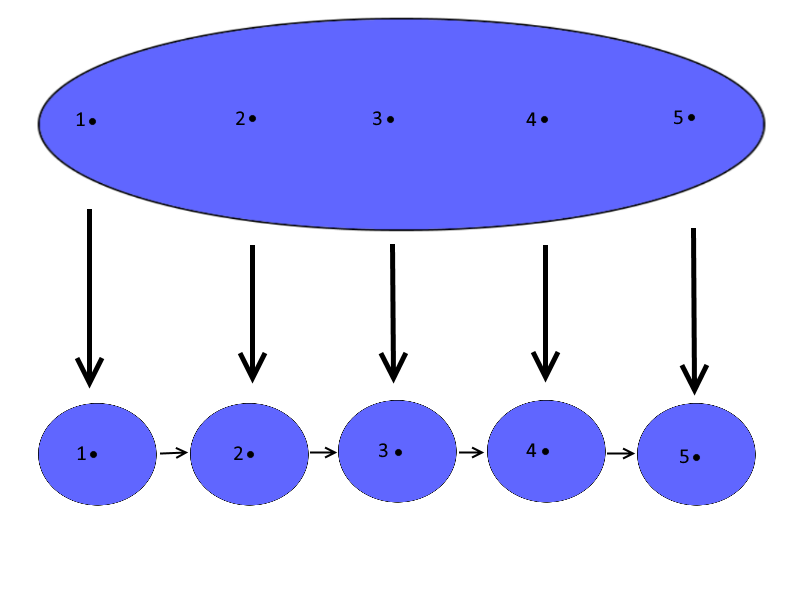
\includegraphics[scale=0.4]{Figures/sliced_salami_method.png}
    \caption{Visualisering av Sliced Salami Method. Et Distributed system deles opp i lumped systems.}
    \label{fig:Sliced_salami}
\end{figure}

\subsection{Numerisk approksimasjon}\label{sec:numerisk_approksimasjon}
En annen metode trekker deg tilbake til vårsemesteret og faget Matte 4N. Vi starter med å dele systemet vårt inn i et grid med punkter som spenner over rommet i de retninger hvor de intensive variablene varierer. 
\begin{figure}[H]
    \centering
    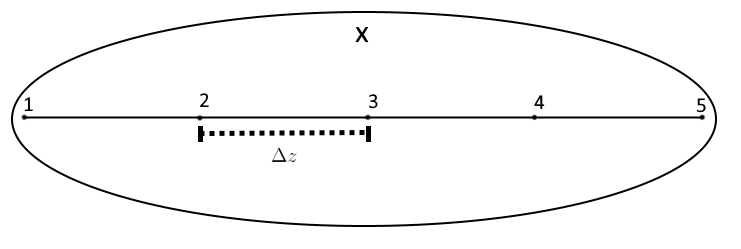
\includegraphics[scale=0.5]{Figures/Distributed_discret.png}
    \caption{Distributed system med intensiv variabel $x$, delt opp i et 1-dimensjonalt grid med 5 punkter og steglengde $\Delta z$.}
    \label{fig:distributed_numerisk}
\end{figure}

I \cref{fig:distributed_numerisk} ser vi at variabelen $x$ endres fra posisjon 1 til posisjon 5. Vi har mange måter å approksimere endringen av $x$ langs $z$ og de fleste bygger på en Taylor utvidelse. Uten å bruke tid på å argumentere for hvorfor dette fungerer setter vi opp en Taylor utvidelse som evaluerer $i+1$ fra posisjon $i$ med lengde $\Delta z$:

\begin{align}
    x_{i+1} = x_i + \frac{dx_i}{dz}\Delta z + \frac{1}{2!}\frac{d^2x_i}{dz^2}(\Delta z)^2 + \frac{1}{3!}\frac{d^3x_i}{dz^3}(\Delta z)^3 + \dots
\end{align}

Litt skummel formel, men likevel nyttig å kunne (pst, dette er fra Matte 1 om du ikke husker). Som oftest i numeriske approksimasjoner benytter vi oss kun av de to første leddene:
\begin{align}
    x_{i+1} &\approx x_i + \frac{dx_i}{dz}\Delta z\\
    &\downarrow \\
    \frac{dx_i}{dz} &\approx \frac{x_{i+1}-x_i}{\Delta z}
\end{align}
Nå som vi har en approksimering for $\frac{dx_i}{dz}$ kan vi sette denne inn for ukjente differensialer, e.g. transportligninger. Approksimeringen vi har i ligningen over er navngitt \textit{Forward method} og er forhåndsvis enkel å bruke. Under har vi lagt fram de vi mener er viktigste numeriske metodene for approksimering av differensialer. 

\begin{equation}
    \begin{split}
    \label{eq:numerical_approx}        
    \text{Forward method: }\frac{dx}{dz}\Big|_i &\approx \frac{x_{i+1}-x_i}{\Delta z} \\
    \text{Central method 1th order: }\frac{dx}{dz}\Big|_i &\approx \frac{x_{i+1}-x_{i-1}}{2\Delta z}\\
    \text{Central method 2th order: }\frac{d^2x}{dz^2}\Big|_i &\approx \frac{x_{i-1}-2x_i+x_{i+1}}{(\Delta z)^2}
    \end{split}
\end{equation}
    

\subsection{Numeriske skjemaer}
Med den numeriske approksimasjonen kan vi substituere ligningene fra (\ref{eq:numerical_approx}) inn i en differensial ligning slik at vi kan benytte oss av programmering til å løse problemet. Uten å bruke for mye tid og krefter på å forklare dette trekker vi fram et enkelt eksempel.

\subsubsection{Eksempel: Euler's method}

\begin{equation}
    \frac{dx}{dz} = e^x + ln(z)  
\end{equation}

Vi setter inn Forwards method for differensialet så ligningen kan løses eksplisitt for $x_{i+1}$.
\begin{align}
    \frac{x_{i+1}-x_i}{\Delta z} &= e^{x_i} + ln(z_i)  \\
    &\downarrow \\
    \label{eq:eulers_methdo_example}
    x_{i+1} = x_i +\Delta z(e^{x_i} + ln(z_i))&, \hspace{1cm} z_{i+1} = z_i + \Delta z
\end{align}
Dette kan vi implementere i python og løse alle $x_i$ ved bruk av forrige $x$ og $z$.

Istedet for å substituerer approksimasjonen av differensiallignignen, som vi gjorde over kan du istedet formulere differensialet på formen:
\begin{equation}
     \frac{dx}{dz} = f(x,z)
\end{equation}

På denne formen kan vi benytte oss av forskjellige numeriske sjemaer som vist under. Siden numerikk ikke er en stor del av pensum i prossmod trekker vi bare fram to metoder for å løse første ordens differensialligninger. 
\begin{align}
    \label{eq:numerical_schemes}
    \text{Eulers method: } x_{i+1} =& x_{i} + \Delta z f(x_i,z_i) \\[0.3cm]
    \text{Heun's method: }x_{i+1} =& x_i + \frac{1}{2}\Delta z[f(x_i,z_i)+f(x_{i+1}^p,z_{i+1}^p)] \\
    x_{i+1}^p =& x_{i} + \Delta z f(x_i,z_i)
\end{align}

\textbf{Ekstra:}\\
Hvorfor skal man bruke det ene skjemaet over det andre spør du? Det har å gjøre med konvergeringen og nøyaktigheten til det numeriske skjemaet. Siden dette er approksimeringer vil den numeriske løsningen avvike fra den ekte løsningen. Avhengig av problemet vi står ovenfor vil en metode være bedre enn en annen. I forskjellige tilfeller vil et skjema gi en rask løsning hvor av et annet skjema ikke vil gi en løsning i det hele tatt (Hvis du synes dette er nyttig og vil lære mer, anbefaler vi å ta faget TKT4140, numeriske beregninger, senere i studiet).  



\clearpage
\section{Shell balance}\label{sec:shell_balance}
En skallbalanse eller ``shell balance'' er en måte å sette opp differensiallikninger som kan brukes til å beskrive hva som skjer i en prosess. Dette gjøres ved å utføre en balanse over en liten bit av system (en ``unit cell''), typisk et lite volum. Herifra antar vi at balansen som gjelder over den lille biten av system også gjelder for hele systemet vi ser på. En slik balanse er basert på balansen vi introduserte i \cref{sec:massetransport}:
\begin{equation}
    \label{eq:gen_balance}
    \text{Akkumulert} = \text{Strøm inn} - \text{Strøm ut} + \text{Generert}
\end{equation}

Når vi setter opp likninger som beskriver det som skjer i en prosess, bruker vi ofte generelle likninger som vi forenkler (eg. Governing equation og Navier Stokes). Dette kan noen ganger være en ganske tungvint måte å gjøre det på, og en shell balance kan da være et godt alternativ for å finne fram til de nødvendige likningene. 

\subsection{Eksempel: Massestrøm gjennom en reaktor med reaksjon}
La oss tenke oss at vi ser på en massestrøm gjennom en reaktor. Vi er da interessert i å se på hvordan systemet endrer seg langs reaktoren. Det første vi kan gjøre er å bestemme oss for en unit cell vi ønsker å gjøre balansen over. I dette tilfellet vil et naturlig valg av en slik unit cell være volumet mellom to tverrsnittsareal i røret. 
\begin{figure}[H]
    \centering
    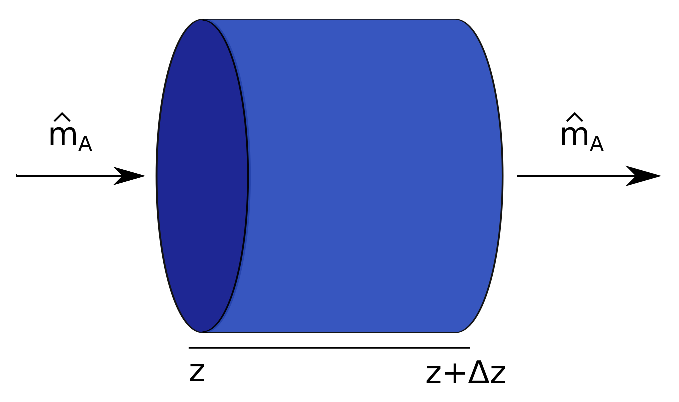
\includegraphics[scale=0.8]{Figures/reactor.eps}
    \caption{Shell balance over et lite volum i en reaktor. A kommer inn i posisjon $z$, reagerer gjennom reaktoren over lengden $\Delta z$ og går ut i posisjon $z+\Delta z$.}
    \label{fig:shell_balance}
\end{figure}

La oss anta at følgende reaksjon skjer gjennom røret: \ce{A ->[\xi_A] B}\\
Videre, la oss sette opp balansen basert på komponent A (merk at vi også kunne satt opp balansen basert på komponent B). Ved å ta i bruk den generelle balansen i \cref{eq:gen_balance} kan en shell balance settes opp på følgende måte:
\begin{equation}
\begin{split}
\label{eq:shellbal}
    \overbrace{\frac{\partial m_A}{\partial t}}^{\text{Akkumulert}} = \overbrace{A \cdot \hat{m}_A\big|_z}^{\text{Inn}} - \overbrace{A \cdot \hat{m}_A\big|_{z+\Delta z}}^{\text{Ut}} - \overbrace{\underbrace{A \cdot \Delta z}_\text{$\Delta V$} \cdot \xi_A}^{\text{Generert}} 
\end{split}
\end{equation}
   Det kan hjelpe å se på benevningnene til utrykkene når du jobber med shell balance for å forstå hvordan du setter opp leddene. Merk at $\hat{m}_A$ er fluksen av masse gjennom tverrsnittsarealet i $z$ eller $z + \Delta z$ . For at du ikke skal forvirres av likningen går vi gjennom hvert ledd:
   
%\begin{align*}
%    \frac{\partial m_A}{\partial t}:&\, \text{Endring av }m_A\text{ inne i kontrollvolumet}\\
%    A \cdot \hat{m}_A\big|_z:&\, \text{ Transport av A inn til kontrollvolumet ved posisjon }z\text{ ganget med tverrsnitt arealet (A)} \\
%    A \cdot \hat{m}_A\big|_{z+\Delta z}:&\, m_A \text{ Transport av A ut av kontrollvolumet ved posisjon }z+\Delta z \text{ ganget med tverrsnitt arealet (A)} \\
%     A\cdot \Delta z \cdot \xi_A:&\, \text{Tap eller generering av A inne i kontrollvolumet ganget med volumet av unit cellen} 
%\end{align*}
\begin{center}
    \begin{tabular}{c c}
     $\frac{\partial m_A}{\partial t}$:    & \makecell{\text{Endring av }$m_A$\text{ inne i kontrollvolumet}} \\[0.4cm]
     $A \cdot \hat{m}_A\big|_z$: & \makecell{\text{ Transport av A inn til kontrollvolumet ved posisjon }$z$\text{ ganget \\ med tverrsnitt arealet (A)}} \\[0.4cm]
      $A \cdot \hat{m}_A\big|_{z+\Delta z}$: & \makecell{\text{ Transport av A ut av kontrollvolumet ved posisjon }$z+\Delta z$ \text{  \\ ganget med tverrsnitt arealet (A)}} \\[0.4cm]
      $A\cdot \Delta z \cdot \xi_A$: & \makecell{\text{Tap eller generering av A inne i kontrollvolumet ganget \\ med volumet av unit cellen}}
    \end{tabular}
\end{center}
Likningen vi har nå satt har et variaber som er definert i posisjon $z$ og $z + \Delta z$. Som oftest har vi ikke kjennskap til posisjonen $z + \Delta z$ og vi må finne en måte å eliminere $\hat{m}_A\big|_{z+\Delta z}$ fra likningen vår.
Vi har i hovedsak to metoder vi kan benytte oss for å få en løsbar likning:
\begin{itemize}
    \item Definisjon av den deriverte
    \item Taylorrekke
\end{itemize}
Definisjonen av den deriverte går ut på å hente ut den matematiske definisjonen av derivasjon fra balansen så vi kan substituere differensiallikninger. I dette kompendiet har vi valgt å gå fram med Taylor utvidelse siden vi har alt brukt den i \cref{sec:distributed}. Vi bruker en Taylorrekke på \cref{eq:shellbal} til å approksimere $\hat{m}_A\big|_{z+\Delta z}$. Dette kan gjøres ved å approksimere posisjon $z+\Delta z$ ved bruk av den deriverte i posisjon $z$. Når vi bruker en Taylorrekke til dette, benytter vi oss av samme metode som i \cref{sec:numerisk_approksimasjon} og bruker kun de to første leddene i rekken, til og med den første deriverte:
\begin{equation}
    \label{eq:shell_lin}
    \hat{m}_A\big|_{z+\Delta z} \approx \hat{m}_A\big|_z + \frac{\partial \hat{m}_A}{\partial z}\Big|_z \cdot \Delta z
\end{equation}
Ved å kombinere \cref{eq:shellbal} og \cref{eq:shell_lin} blir balansen enklere å jobbe med siden alle variablene er i posisjon $z$. Notasjonen $\big|_z$ sløyfes herfra for enkelhetens skyld. 
\begin{equation}
    \label{eq:shell_bal_2}
    \frac{\partial m_A}{\partial t} = A \cdot \left(\hat{m}_A - \hat{m}_A - \frac{\partial \hat{m}_A}{\partial z} \cdot \Delta z \right) - \Delta V \cdot r_A
\end{equation}
Her bør det merkes at $\Delta V = A \cdot \Delta z$. Herifra kan vi forenkle likningen, for så og dele på $\Delta V$. Ved å la $\rho_A = m_A/V$ får vi en massebalanse gjennom røret:
\begin{equation}
    \label{eq:final_balance}
    \frac{\partial \rho_A}{\partial t} = \frac{\partial \hat{m}_A}{\partial z} - r_A
\end{equation}
I dette eksemplet burde det merkes at $r_A [=] \frac{kg}{s \cdot m^3}$. For en (litt) mer detaljert forklaring på hvordan vi går fra likning \cref{eq:shell_bal_2} til \cref{eq:final_balance} anbefales det å se ABC-heftet Avsnitt 4.


\clearpage
\section{Blokkdiagrammer og The Grand Scheme}\label{sec:signal_block_diagram}
I alle fag frem til nå har du sett på et flytdiagram med piler og bokser og tenkt at dette er masse som beveger seg fra en tank til en annen. Ta eksempelet gitt i \cref{fig:simple_blockdiagram}. Hadde vi spurt en kybernetiker hadde han beskrevet figuren som en oversikt over informasjonsflyten til systemet. Som prosessingeniør er det viktig å vite forskjellenene mellom blokkdiagram og flytskjema og deres respektive bruksområder.

\begin{figure}[H]
    \centering
    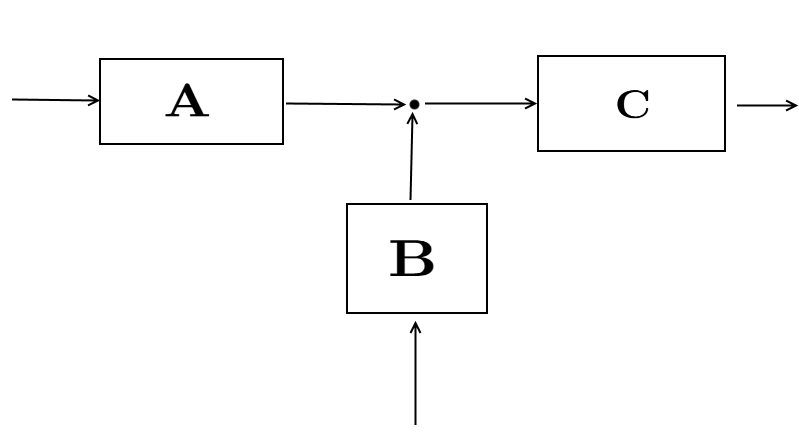
\includegraphics[scale=0.5]{Figures/simple_blockdiagram1.png}
    \caption{Et blokkdiagram.}
    \label{fig:simple_blockdiagram}
\end{figure}

\subsection{Blokkdiagram}
Et blokkdiagram er en visualisering av signaler som sendes fra et system til andre systemer. Til forskjell fra flytskjema er pilene i et blokkdiagram signaler som bærer informasjon istedet for masse. Ved å bruke et blokkdiagram kan vi visualisere hvordan systemer kommuniserer med hverandre i form av lineære sammenhenger.

\begin{figure}[H]
    \centering
    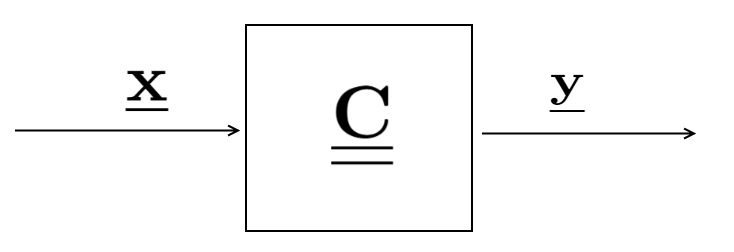
\includegraphics[scale=0.5]{Figures/very_simple_blockdiagram.png}
    \caption{Et veldig enkelt blokkdiagram}
    \label{fig:very_simple_blockdiagram}
\end{figure}

Blokkdiagrammet i \cref{fig:very_simple_blockdiagram} viser den lineære sammenhengen mellom $\underline{\textbf{x}}$ og $\underline{\textbf{y}}$, som kan beskrives som ligningen: 
\begin{equation}
    \label{eq:very_simple_blokkdiagram}
    \underline{\textbf{y}} = \doubleunderline{\textbf{C}}\,\underline{\textbf{x}}
\end{equation}
Trikset med blokkdiagrammer er at alle variablene/vektorene/matrisene ganges med hverandre via en pil og plusses sammen hvis pilen møter en annen pil. Det er mange måter å angripe et blokkdiagram, men en enkel metode er å starte bakerst og bevege deg mot pilens retning. Da er du sikker på at du får riktig plassering på vektorer og matriser.

\begin{figure}[H]
    \centering
    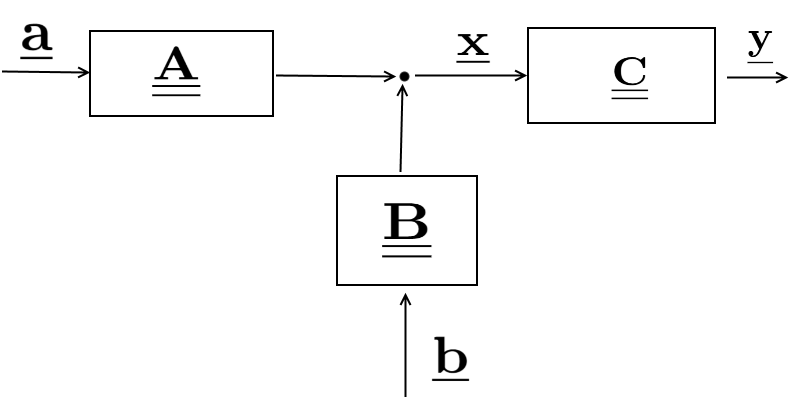
\includegraphics[scale=0.5]{Figures/simple_blockdiagram.png}
    \caption{Blokk diagram med 3 systemer hvor signalet \textbf{y} er en lineær kombinasjon av signalene \textbf{a} og \textbf{b}.}
    \label{fig:simple_blokkdiagram1}
\end{figure}

Fra \cref{fig:simple_blokkdiagram1} er det to likninger vi kan hente ut. Den første er den samme som i \cref{eq:very_simple_blokkdiagram} og den andre er den lineær kombinasjonen mellom $\doubleunderline{\textbf{A}}\,\underline{\textbf{a}}$ og $\doubleunderline{\textbf{B}}\,\underline{\textbf{b}}$:

\begin{align}
       \label{eq:simple_blokkdiagram}
    \underline{\textbf{y}} =& \doubleunderline{\textbf{C}}\,\underline{\textbf{x}} \\
    \underline{\textbf{x}} =& \doubleunderline{\textbf{A}}\,\underline{\textbf{a}} + \doubleunderline{\textbf{B}}\,\underline{\textbf{b}}
\end{align}

\subsection{The Grand Scheme}
The Grand Scheme er hele pensum summert opp. Tanken bak The Grand Scheme er at man kan koble sammen alle delene i modellering til et blokkdiagram. I ABC-heftet blir The Grand Scheme forklart ved et blokkdiagrammet gitt i \cref{fig:grand_scheme_hard}:

\begin{figure}[H]
    \centering
    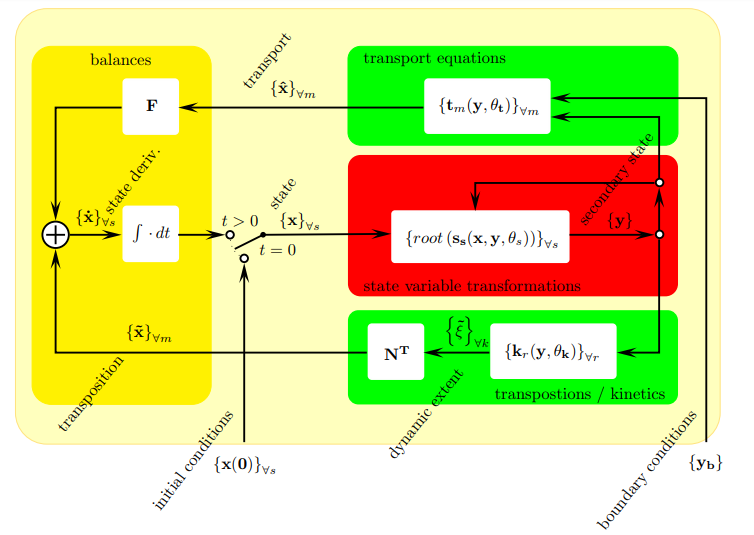
\includegraphics[scale=0.7]{Figures/The_grand_scheme_hard}
    \caption{The Grand Scheme, hentet fra ABC-heftet.}
    \label{fig:grand_scheme_hard}
\end{figure}

Siden dette blokkdiagrammet er litt vanskelig å skjønne har vi laget en versjon som er litt mindre korrekt, men litt mer lesbar når man først introduseres til The Grand Scheme.

\begin{figure}[H]
    \centering
    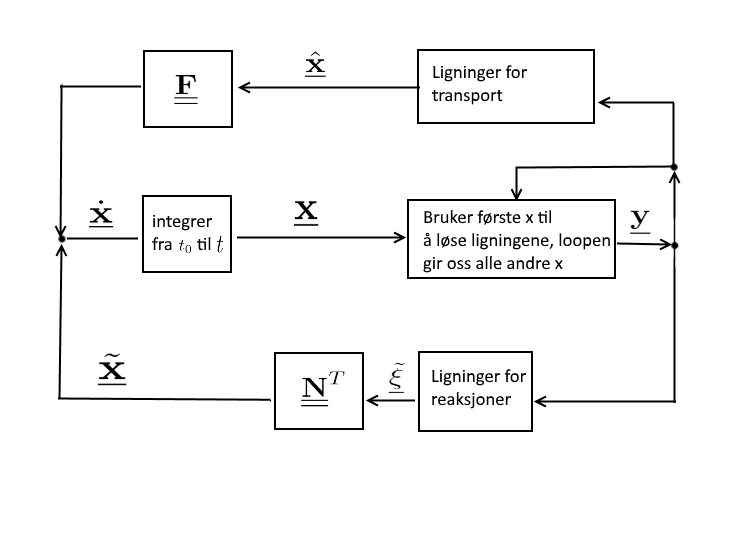
\includegraphics[scale=0.7]{Figures/The_grand_scheme_enkel.png}
    \caption{The Grand Scheme, forenklet.}
    \label{fig:grand_scheme_enkel}
\end{figure}

Bruker vi det vi har lært om blokkdiagrammer og tyder \cref{fig:grand_scheme_hard} i form av linære kombinasjoner får vi et sett med ligninger som beskriver det essensielle i prossmod. Under er $f,g,h$ funksjoner for henholdsvis state, reaksjoner og transport. 

\begin{equation}
\label{eq:The_grand_scheme}
    \begin{split}
    \vecdot{x} =&\, \mymat{F}\,\vechat{x} + \vectil{x} \\
    \vectil{x} =&\, \mymat{N}^T\,\Tilde{\underline{\xi}} \\
    \Tilde{\underline{\xi}} =&\, g(\vec{y}) \\
    \vechat{x} =&\, h(\vec{y}) \\
    \vec{x}_{\text{next state}} &=\, f(\vec{y}) 
    \end{split}
\end{equation}
    
Likningene over kjenner du forhåpentligvis igjen fra tidligere kapitler. Det er ikke så mye mer å si om The Grand Scheme enn at mesteparten av pensum kan summeres opp i det. 


\clearpage
\section{Reduksjon av modeller med time scale og kapasitet}\label{sec:timescale}
En modell er alltid bygget på et sett med antagelser som divergerer modellen fra det reelle. Frem til nå har vi gjort antagelser på kapasitet og time scale uten å være fullt klar over argumentene for antagelsene. Time scale assumptions er kort fortalt neglisjering av modeller pga dynamiske forskjeller. Vi kan dele en time scale inn i tre deler:


\begin{itemize}
    \item Event dynamic: Skjer  umiddelbart
    \item Dynamisk: Forandring over tid som er merkbart
    \item Konstant: Ingen forandring i system
\end{itemize}

\begin{figure}[H]
    \centering
    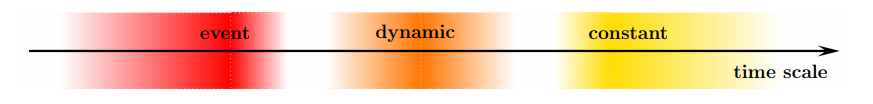
\includegraphics[scale=0.5]{Figures/time_scale}
    \caption{Time scale som visualiserer hvordan event, dynamic og constant henger sammen. Merk at ingen av domenene overlapper.}
    \label{fig:time_scale}
\end{figure}


Vi har mange måter å gå fram på for å redusere modeller. Vi bruker i hovedsak 4 angrepsvinkler. De fire forskjellige metodene blir nærmere forklart i det kommende eksempelet i \cref{sec:tre_sjo}. 
\begin{enumerate}
    \label{lst:reduction}
    \item Ekspandere det som er konstant
    \item Introdusere event dynamic
    \item Analysere den raske dynamikken
    \item Analysere den trege dynamikken
\end{enumerate}

\subsection{Eksempel: Tre innsjøer}\label{sec:tre_sjo}
Vi ønsker å modellere vannet som renner fra en stor innsjø (R) til en mindre (C) og videre til en enda mindre innsjø (S). For å forklare reduksjonen best mulig trekker vi fram en enkel topologi:


\begin{figure}[H]
    \centering
    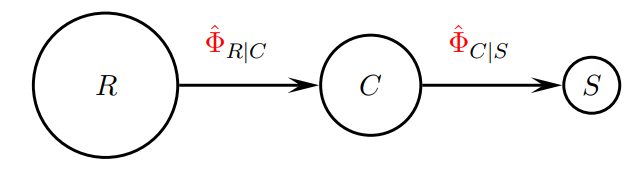
\includegraphics[scale=0.5]{Figures/time_scale_topo}
    \caption{Topologi for tre innsjøer hvor R transporterer til C som transporterer til S.}
    \label{fig:time_scale_topo}
\end{figure}

Den fulle modellen for topologien for \cref{fig:time_scale_topo} gir ligningene:
\begin{align}
    \dot{\Phi}_{R} =&\, -\hat{\Phi}_{R|C} \\
    \dot{\Phi}_C =&\, \hat{\Phi}_{R|C} - \hat{\Phi}_{C|S}\\
    \dot{\Phi}_S =&\, \hat{\Phi}_{C|S}
\end{align}

Vi gjør reduksjon ved bruk av de fire angrepsvinklene. I ABC-heftet kapittel 16 har de en matematisk forklaring på reduksjonen, den har vi valgt å ikke ta med til fordel for den intuitive forklaringen.  

\begin{center}
    \textbf{1:} Ekspandere det som er konstant.
\end{center}
Ved å anta at R er mye større enn C og S så kan vi observere R som et reservoar som fører til at vi ikke trenger å modellere R ($\underline{\dot{\Phi}}_R = 0$).

\begin{figure}[H]
    \centering
    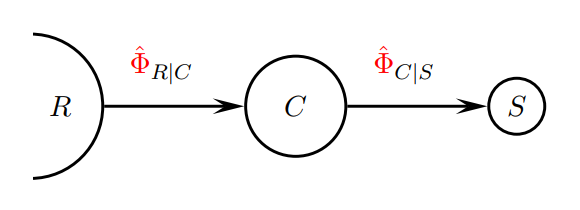
\includegraphics[scale=0.5]{Figures/time_scale_topo1.png}
    \caption{Topologi for tre innsjøer hvor R er betydelig mye større enn C og S.}
    \label{fig:time_scale_topo1}
\end{figure}
Dette gir oss en ny modell:
\begin{align}
    \dot{\Phi}_C =&\, \hat{\Phi}_{R|C} - \hat{\Phi}_{C|S}\\
    \dot{\Phi}_S =&\, \hat{\Phi}_{C|S}
\end{align}


\begin{center}
    \textbf{2:} Introdusere event dynamic.
\end{center}

Hvis vi antar at volumet S er minimalt forhold til C, kan vi anta at det som går ut av C til S er neglisjerbart forhold til transporten fra R til C.

\begin{figure}[H]
    \centering
    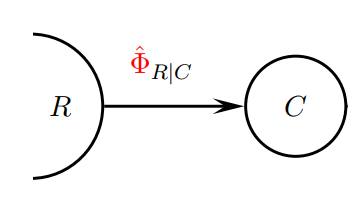
\includegraphics[scale=0.5]{Figures/time_scale_topo2.png}
    \caption{Topologi for tre innsjøer hvor transporten fra C til S er så minimal at det ikke har noen påvirkning på modellen.}
    \label{fig:time_scale_topo2}
\end{figure}



\begin{center}
    \textbf{3:} Analysere den raske dynamikken (small time scale).
\end{center}

Vi tar fram topologien i \cref{fig:time_scale_topo1}, etter ekspansjonen av det konstante domenet, og setter inn en lineær modell for transport som vi lærte i \cref{sec:linear_transport}.

\begin{align}
    \dot{\Phi}_C =&\, \hat{\Phi}_{R|C} - \hat{\Phi}_{C|S}\\
    \dot{\Phi}_S =&\, \hat{\Phi}_{C|S} \\[0.5cm]
    \dot{\Phi}_C =&\, -k_{R|C}(\pi_C-\pi_R) +k_{C|S}(\pi_S-\pi_C)\\
      \dot{\Phi}_S =&\ -k_{C|S}(\pi_S-\pi_C)
\end{align}

Ved å anta at transporten $\hat{\Phi}_{R|C}$ er mye tregere enn  $\hat{\Phi}_{C|S}$ kan vi anta at ved en liten timescale vil $\hat{\Phi}_{C|S}$ dominere og vi kan neglisjere transporten fra R til C i $\dot{\Phi}_C$:

\begin{align}
    \dot{\Phi}_C =&\, +k_{C|S}(\pi_S-\pi_C)\\
      \dot{\Phi}_S =&\ -k_{C|S}(\pi_S-\pi_C)
\end{align}

\begin{center}
    \textbf{4:} Analysere den trege dynamikken (large time scale).
\end{center}

Å bruke en lang time scale er veldig vanlig i prosessmodellering. Etter en lang tid vil forskjellen i effort variabler, mellom de to systeme, forsvinne. Tenk deg at du har laget deg en kopp med varm kaffe. Venter du i 24 timer før du drikker kaffen kan du forvente at temperaturen til koppen er den samme som rommet. 

\begin{align}
    0 =&\, k(\pi_S - \pi_C) \\
    \pi_C =&\, \pi_S
\end{align}
\clearpage
\section{Programmering}\label{sec:prog}
Programmering i prosessmodellering er utfordrende på flere plan. For det første er det forventet at du kan en del av det du har lært i ITGK, prosessteknikk og tidligere mattefag. Hvis du ikke husker disse metodene anbefaler vi deg å lese deg opp på dette før du begynner på programmeringsdelen. I prossmod er det forventet at du skal kunne bruke numerikk til å løse sett med ODE (Ordinary Differational Equations). I tillegg er det forventet at diverse problemer av skal gjøres objektorientert. Dette kan være utfordrende og krever en del tid, men vi skal prøve å guide deg gjennom de viktigste punktene i objektorientert programmering. Hvis du greier å lære deg dette har du et stort fortrinn til vårfaget TDT4102 - Prosedyre- og objektorientert programmering (C++), som vi anbefaler enhver student på IKP å ta.

 %\subsection{Løse ODE med programmering}
 
% Fra \cref{sec:numerisk_approksimasjon} lærte vi hvordan man approksimerte en differensialligning med bruk av Taylor utvidelser. tilstanden i punkt $i+1$ kan ofte beregnes hvis vi vet tilstanden i punkt $i$. For at dette skal komme litt tydeligere fram ser vi tilbake til eksempelet fra \cref{sec:euler_numerical}. Fra eksempelet bruke Forwards method til å komme fram til to eksplisitte ligninger hvor $x_{i+1}$ ble beregnet fra $x_i$ og $z_i$.

% \begin{align}
%     \label{eq:eulers_methdo_example2}
%     x_{i+1} = x_i +\Delta z(e^{x_i} + \ln (z_i))&, \hspace{1cm} z_{i+1} = z_i + \Delta z
% \end{align}

% Ligningene vi har nå er perfekt å putte inn i et programmeringsspråk. Dette er fordi at vi kan loope over alle posisjonene $i$ for å finne ut hva x er i en posisjon. La oss si at $x$ er \textcolor{red}{isdhfsd} og z er posisjonen i en reaktor hvor $z_{start}$ er start og $z_{slutt}$ er enden av reaktoren. Vi starter med å initialiserer de variablene vi vet. I dette eksempelet sier vi at reaktoren er 5 meter lang og at vi ønsker beregne 100 posisjoner i reaktoren. 

% \textbf{Del 1 (Kode):}
% \begin{lstlisting}[language=python]
% class Katt: #Klassen katt
%     #Medlemsvariabler
%     antall_ben = 4 
%     navn ="" #Default navn
    
%     #Constructor
%     def __init__(self, navn): #Lager Katte-objektet med spesifisert navn
%         self.navn = navn #Endrer navnet til katten fra "" til det vi spesifiserte

% \end{lstlisting}

\subsection{Klasser og objekter}
Til nå har dere ofte programmert i en fil med definering av variabler øverst i filen og så skrevet viktige funksjonener under. I IT-verdenen er dette kronglete siden et program kan trenge flere titusen linjer med koder så vi må ha et system for å sortere koden. Samtidig vil operasjoner i programmet gjenta seg og vi ønsker ikke å skrive en kode flere ganger. Av den grunn er objektorientert programmering fantastisk siden vi kan generalisere hvordan en del av koden skal oppføre seg i forhold til en annen del. Formelt sett er klasser et overordnet rammesystem for hvordan objekter kommuniserer sammen. Det kan være alt fra hvordan en bil ser ut til hvordan et matematisk system fungerer. Før dere blir mer forvirret trekker vi fram et eksempel på klasser og objekter.

\subsubsection{Eksempel: Katter og hunder}
Tenk deg at du har lager et dataspill med en åpen verden og sjefen din ber deg om å fylle verdenen med katter. Du tenker deg om og kommer fram til følgende konklusjon: Alle kattene i denne verdenen har et navn og har fire bein. Istedet for å programmere dette for hver eneste katt lager vi et generelt rammeverk som gjelder alle katter.

\begin{figure}[H]
    \centering
    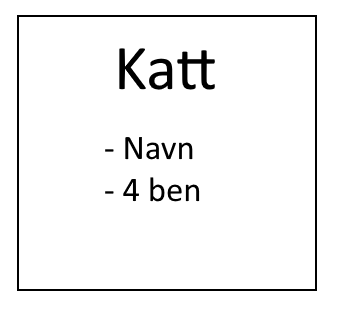
\includegraphics[scale=0.5]{Figures/Klasser_katt.png}
    \caption{En visualisering av klassen $"$Katt$"$.}
    \label{fig:Katte_boks}
\end{figure}

Når vi lager et rammeverk for alle kattene kan vi fylle verdenen vår med mange katteobjekter. Det vil si at i verdenen vår har vi mange forskjellige katte-objekter, men alle katte-objektene tilhører klassen ``Katt'' og hvert katte-objekt vil ha et navn og fire bein. Ved bruk av python som programmeringspråk skriver vi klassen for katt.\\[0.5cm]
\textbf{Del 1 (Kode):}
\begin{lstlisting}[language=python]
class Katt: #Klassen katt
    #Medlemsvariabler
    antall_ben = 4 
    navn ="" #Default navn
    
    #Constructor
    def __init__(self, navn): #Lager Katte-objektet med spesifisert navn
        self.navn = navn #Endrer navnet til katten fra "" til det vi spesifiserte

\end{lstlisting}
\textbf{Del 2 (Konsoll):}
\begin{lstlisting}[language=python]
>>> katten_butte = Katt("Butte") #Lager et katteobjekt med variabelnavn "katten_butte"
>>> print(katten_butte.navn) 
Butte
>>> print(katten_butte.antall_ben) 
4
\end{lstlisting}

En liten forklaring på hva som skjer.

``\twound{init}\twound{\text{ }}(self,navn)'' er en konstruktør for et katte-objekt. init kommer fra det engelske ordet ``initial''. Når vi skal lage et et katteobjekt må vi kalle på konstruktøren vår. Ved å kalle på kontruktøren lager python et tomt objekt og sender det til oss i form av ``self''. Self er på mange måter ``Seg selv'' så når vi bruker self snakker vi om det spesifikke katte-objektet. Konstruktøren tar også inn et navn som vi må spesifisere. Vi kunne ha programmert konstruktøren til å ta inn antall bein også, men siden en katt alltid har 4 bein så gir det ingen mening å la brukeres bestemme hvor mange bein et katte-objekt skal ha. På linje 1 i Del 2 lager vi et objekt som vi kaller ``katten\_butte'' som vi spesifiserer skal ha navnet ``Butte''. Navn og antall bein til katten er en instans av klassen vår. Det vil si ``Egenskaper'' til katte-objektet. Her er det viktig å skille mellom variabelnavnet på objektet og instansen til objektet som er vi har valgt å kalle ``navn''.

Sjefen vår er ikke helt fornøyd med at spillverdenen bare består av katter. Han ber oss om å legge til hunder i tillegg til kattene og hundene skal kunne bjeffe.

\begin{figure}[H]
    \centering
    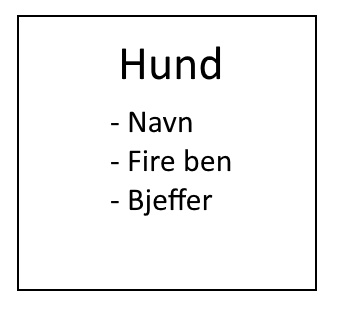
\includegraphics[scale=0.5]{Figures/Klasser_hund.png}
    \caption{En visualisering av klassen ``Hund''.}
    \label{fig:klasse_hund}
\end{figure}

Hunden har de samme medlemsvariablene som en katt, men skal i tillegg ha medlemsfunksjonen å bjeffe. Dette gjør vi ved å lage det som kalles en medlemsfunksjon til klassen. En funksjon som bare klassen $"$Hund$"$ kan benytte seg av.\\[0.5cm]
\textbf{Del 1 (Kode):}
\begin{lstlisting}[language=python]
class Hund: #Klassen Hund
    #Medlemsvariabler
    antall_ben = 4 
    navn ="" #Default navn
    
    #Constructor
    def __init__(self, navn): #Lager hunde-objektet med spesifisert navn
        self.navn = navn #Endrer navnet til hunden fra "" til det vi spesifiserte
    #Medlemsfunksjon
    def bjeffe(self): 
        print("BARK BARK")
\end{lstlisting}
\textbf{Del 2 (Konsoll):}
\begin{lstlisting}[language=python]
>>> Hunden_tara = Hund("Tara") #Lager et Hundeobjekt med variabelnavn "Hunden_tara"
>>> print(Hunden_tara.navn) 
Tara
>>> Hunden_tara.bjeffe() #Kaller bjeffefunksjonen
BARK BARK
\end{lstlisting}

Nå har vi en klasse for Hund og for Katt som alle objekter i spillverdenen vår må følge. En klasse er et strengt rammeverk i form av at et objekt ikke kan gjøre annet enn det klassen tillater. Det vil si at hvis vi prøver å skrive katten\_butte.bjeffe() så får vi feilmelding siden klassen Katt, som katten\_butte er et objekt av, ikke har en funksjon som heter bjeffe(). 

\clearpage
\subsection{Superklasser, subklasser og arv}
I mange tilfeller vil man ha klasser som har de samme medlemsvariablene og samme medlemsfunksjonene. Istedet for å definere de samme funksjonene til hver klasse er det smartere å la en klasse arve medlemsfunksjoner og medlemsvariabler fra det vi kaller en superklasse. 

\subsubsection{Eksempel: Mange forskjellige dyr}
Sjefen vår kommer inn og sier at vi også skal ha kuer, griser, hester og mange andre forskjellige dyr i spillverdenen vår. Vi oppdager at dette blir mye repetisjon av kode som vi må spesifisere for hver klasse. Hund og katt hadde begge 4 ben og et navn. Her kan vi koble disse to klassene til en superklasse som vi kaller Dyr. Hund og Katt blir da subklasser av superklassen Dyr.\\[2cm]

\begin{figure}[H]
    \centering
    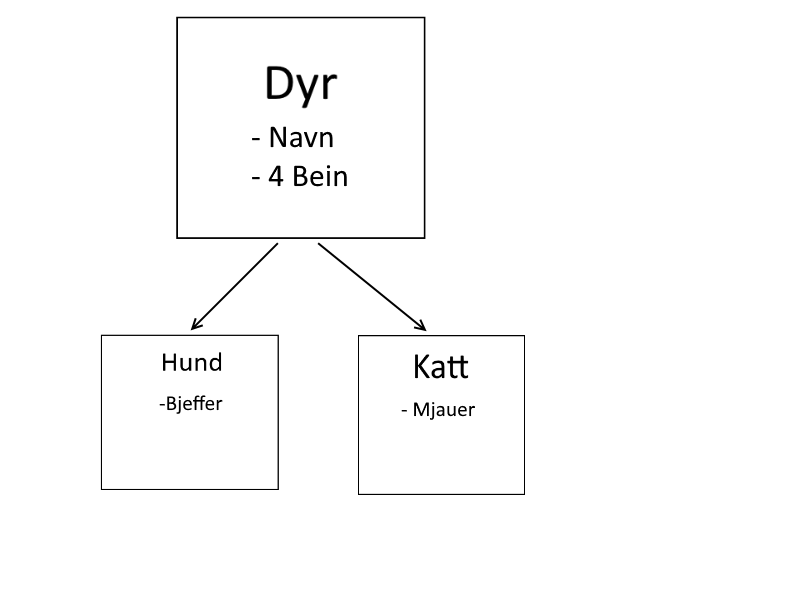
\includegraphics[scale=0.5]{Figures/Klasser_Dyr.png}
    \caption{En visualisering av superklassen Dyr med Katt og Hund som subklasser.}
    \label{fig:uperklasse}
\end{figure}
\clearpage
\begin{lstlisting}[language=python]
class Dyr(): # Klassen Dyr
    #Medlemsvariabler for alle dyre-objekter
    antall_ben = 4
    navn = ""
    #Contructor for dyre-objekter
    def __init__(self, navn):
        self.navn = navn

class Katt(Dyr): # Klassen Katt, arver fra klassen Dyr
    #Medlemsfunksjoner
    def mjaue(self):
        print("MJAAAAU")
        
    def __init__(self,navn): #Spesifiserer construktor for Katte-klassen
        super().__init__(self,navn) #Kaller superklassen sin constructor


class Hund(Dyr):  # Klassen Hund, arver fra klssen Dyr
    #Medlemsfunksjon
    def bjeffe(self):
        print("BARK BARK")
\end{lstlisting}

Som du ser i koden over så har klassen Katt en spesifisert konstruktør mens Hund har ingen. I realiteten er det ingen forskjell mellom klassene siden linje 15 kaller på konstruktøren til Dyr hvorav Katt vil automatisk kalle på konstruktøren. Denne kalles automatisk siden Katt arver konstruktøren til klassen Dyr. Vi valgte å ta med linje 14 og 15 for å vise deg hvordan du kan definere din egen konstruktører for subklasser. Dette er nyttig å kunne når subklasser skiller seg fra superklasser.

\textbf{Ekstra}: \\
Under er koden for filen $"$Min\_python\_fil.py$"$
\begin{lstlisting}[language=python]
if __name__ == "__main__":
    print("Dette er hovedskriptet")
\end{lstlisting}

Linje 1 i koden over er litt merkelig å forstå, men tanken er at hvis du kaller på den spesifikke filen  $"$Min\_python\_fil.py$"$ så vil betingelsen til if-setningen gi ut True som gjør at linje 2 vil kjøre.

\begin{lstlisting}
>>> python Min_python_fil.py
Dette er hovedskriptet
\end{lstlisting}
 Vi ønsker å gjøre dette er fordi filen kan importeres fra andre filer. Hvis vi kjører en annen fil som importerer  $"$Min\_python\_fil.py$"$, så vil ikke if-betingelsen godkjennes.  


\clearpage
\section{Tabell med de viktigste ligninger}
Under har vi ramset opp de ligningene vi mener du bør huske til eksamen. Dette gjelder ikke nødvendigvis likninger som du har blitt introdusert for i tidligere fag. I tillegg er det viktig å påpeke at noen ligninger, som shell balance, må du lære deg å utlede siden å pugge dem vil sjelden treffe riktig. 
\begin{table}[H]
    \centering
    \begin{tabular}{c|c}
        Totalt akkumulering & $\Phi = \int_{t_0}^{t}\dot{\Phi}\,dt $  \\[0.2cm]
         Balanse  & $\dot{\Phi} = \hat{\Phi}_{inn} - \hat{\Phi}_{ut} + \Tilde{\Phi}$ \\[0.2cm]
         Konservering & $\dot{\Phi} = \hat{\Phi}_{inn} - \hat{\Phi}_{ut} $\\[0.2cm]
         System av transportligninger & $\underline{\dot{\Phi}} = \textbf{\doubleunderline{F}}\hspace{0.1cm}\underline{\hat{\Phi}}$ \\[0.2cm]
         Transport av ekstensiv variabel & $\hat{\varphi} = -c\frac{\partial \pi}{\partial \underline{\textbf{r}}}$ \\[0.2cm]
         Lineær transportligning & $\hat{\Phi}_{a|b} = -k_{a|b}(\pi_a-\pi_b)$ \\[0.2cm] 
         Generering av stoffmenge & $\vectil{n}=\,V\mymat{N}^T\underline{\Tilde{\xi}}(\vec{c})$ \\[0.2cm]
         Kjemisk potensial & $\mu_i =\, \mu_{i}^0 + RT\ln (x_i)$ \\[0.2cm]
         Reaksjonsrate & $\Tilde{\xi} = k^r_r\,g(c)$ \\[0.2cm] 
         Arrhenius ligning & $k^r_r(T) =k^0_r\,e^{\frac{-E_{A}}{RT}}$ \\[0.2cm]
         
         Taylor utvidelse av første orden & $x_{i+1} \approx x_i + \frac{dx_i}{dz}\Delta z$ \\[0.2cm]
    \end{tabular}
    \label{tab:my_label}
\end{table}

\appendix
\section{Referanse}
Heinz A. Presig, \textit{ABC of modelling}, hentet fra TKP4106 \url{http://folk.ntnu.no/preisig/}

\end{document}
